%\section{ Prices for different methods for binary option }\label{appendix:Call prices for different methods_binary}
%
%\begin{table}[h!]
%	\centering
%	\begin{tabular}{l*{6}{c}r}
%		Method \textbackslash  Steps            & $2$ & $4$ & $8$ & $16$ &   \\
%		\hline
%		MISC ($TOl=5.10^{-1}$)  & $\red{0.4619}$ & $  \red{0.4404}$ & $\red{0.4299}$ & $\red{0.4250}$  \\
%		\hline
%	\end{tabular}
%	\caption{ Binary option price of the different methods for different number of time steps, without Richardson extrapolation.}
%	\label{table: Binary option price of the different methods for different number of time steps}
%\end{table}
%
%
%\begin{table}[h!]
%	\centering
%	\begin{tabular}{l*{6}{c}r}
%		Method \textbackslash  Steps   &$1-2$         & $2-4$ & $4-8$ & $8-16$  \\
%		\hline
%		MISC ($TOl=5.10^{-1}$) & $\red{0.4239}$ & $0.4188$ & $  0.4194$ & $0.4200$   \\
%			MISC ($TOl=10^{-2}$) & $-$ & $\red{0.4192}$ & $  0.4194$ & $0.4201$   \\
%			MISC ($TOl=10^{-3}$) & $-$ & $-$ & $  \red{0.4198}$ & $\red{0.4205}$   \\
%		\hline
%	\end{tabular}
%	\caption{Binary  option price of the different methods for different number of time steps, with Richardson extrapolation (level $1$).}
%	\label{table: Binary option price of the different methods for different number of time steps, binary option, with richardson, level 1}
%\end{table}
%
%\newpage
%
%
%\section{ Call prices for different methods}\label{appendix:Call prices for different methods}
%
%\begin{table}[h!]
%	\centering
%	\begin{tabular}{l*{6}{c}r}
%		Method \textbackslash  Steps            & $2$ & $4$ & $8$ & $16$ &   \\
%		\hline
%		MISC ($TOl=5.10^{-1}$)  & $\red{16.2145}$ & $16.1352$ & $\red{16.0275}$ & $\red{15.9594}$  \\
%			MISC ($TOl=10^{-3}$)  & $-$ & $ \red{16.1328 }$ & $-$ & $-$  \\
%		\hline
%	\end{tabular}
%	\caption{ Call option price of the different methods for different number of time steps, without Richardson extrapolation.}
%	\label{table: Call option price of the different methods for different number of time steps}
%\end{table}
%
%
%\begin{table}[h!]
%	\centering
%	\begin{tabular}{l*{6}{c}r}
%		Method \textbackslash  Steps   &$1-2$         & $2-4$ & $4-8$ & $8-16$  \\
%		\hline
%		MISC ($TOl=5.10^{-1}$) & $\red{16.4419}$ & $16.0558$ & $15.9205$ & $15.8915$   \\
%		MISC ($TOl=10^{-3}$) & $-$ & $\red{16.0510}$ & $ \red{15.9177}$ & $\red{15.8880}$   \\
%		\hline
%	\end{tabular}
%	\caption{Call  option price of the different methods for different number of time steps, with Richardson extrapolation (level $1$).}
%	\label{table: Call option price of the different methods for different number of time steps, binary option, with richardson, level 1}
%\end{table}
%
%\begin{table}[h!]
%	\centering
%	\begin{tabular}{l*{6}{c}r}
%		Method \textbackslash  Steps   &$1-2-4$         & $2-4-8$ & $4-8-16$   \\
%		\hline
%		MISC ($TOl=5.10^{-1}$) & $15.9269$ & $15.8756$ & $15.8815$  \\
%		MISC ($TOl=10^{-3}$) & $\red{15.9205}$ & $\red{15.8732}$ & $ \red{  15.8789}$   \\
%		\hline
%	\end{tabular}
%	\caption{Call option price of the different methods for different number of time steps, with Richardson extrapolation (level $2$).}
%	\label{table: Call option price of the different methods for different number of time steps, binary option, with richardson, level 2}
%\end{table}
%\newpage



%
%\section{Results of the basket example}
%\subsubsection{Verifying bounds on work and error contributions}
%
%In this subsection, we discuss the validity of Assumptions $2$-$4$ in \cite{haji2016multi}, upon which the MISC convergence theorem is based. In this case, basket option case we do not use a deterministic solver since the we have a close for of the integrand and then  we analyze  only the properties of the collocation method applied to
%the problem.
%
%
%
%
%Below, we show in figures (\ref{fig:test_basket_1},\ref{fig:test_basket_2},\ref{fig:test_basket_3}) the rate of convergence of first and mixed differences for different orders and we check that the error is decaying exponentially wrt number of points used in the quadrature.
%
%	
%	\begin{figure}[h!]
%		\centering
%		\begin{subfigure}{.5\textwidth}
%			\centering
%			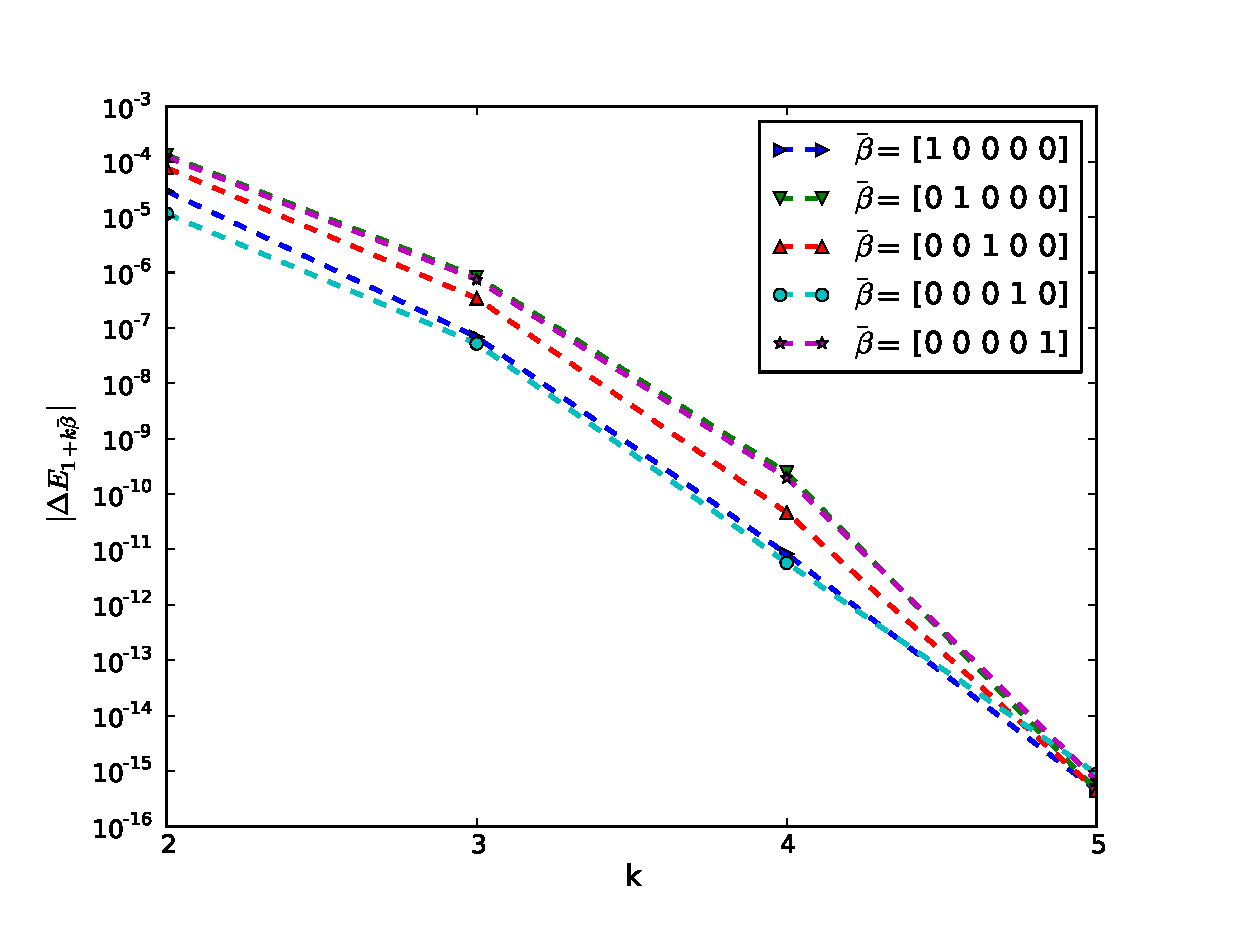
\includegraphics[width=1\linewidth]{./figures/first_difference_basket.eps}
%			\caption{}
%			\label{fig:sub1}
%		\end{subfigure}%
%		\begin{subfigure}{.5\textwidth}
%			\centering
%			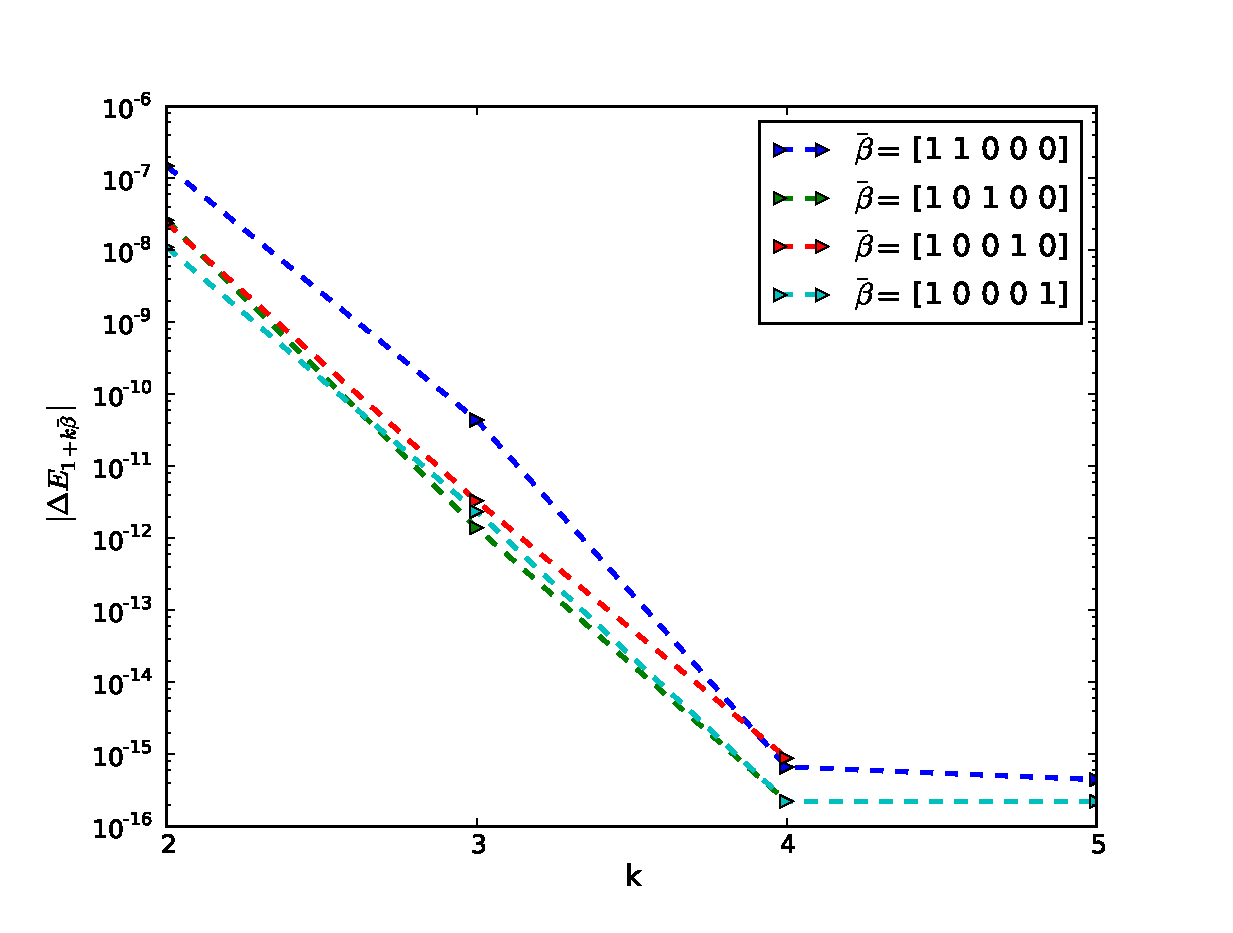
\includegraphics[width=1\linewidth]{./figures/mixed_difference_order2_basket_1.eps}
%			\caption{}
%			\label{fig:sub2}
%		\end{subfigure}%
%		\caption{The rate of convergence of $\abs{\Delta E_{\beta}}$ ($\beta=\mathbf{1}+k \bar{\beta}$): a) shows the rate of convergence of first order differences. b)  shows the rate of convergence of second order mixed differences.}
%			\label{fig:test_basket_1}
%	\end{figure}
%
%	\begin{figure}
%	\centering
%	\begin{subfigure}{.5\textwidth}
%		\centering
%		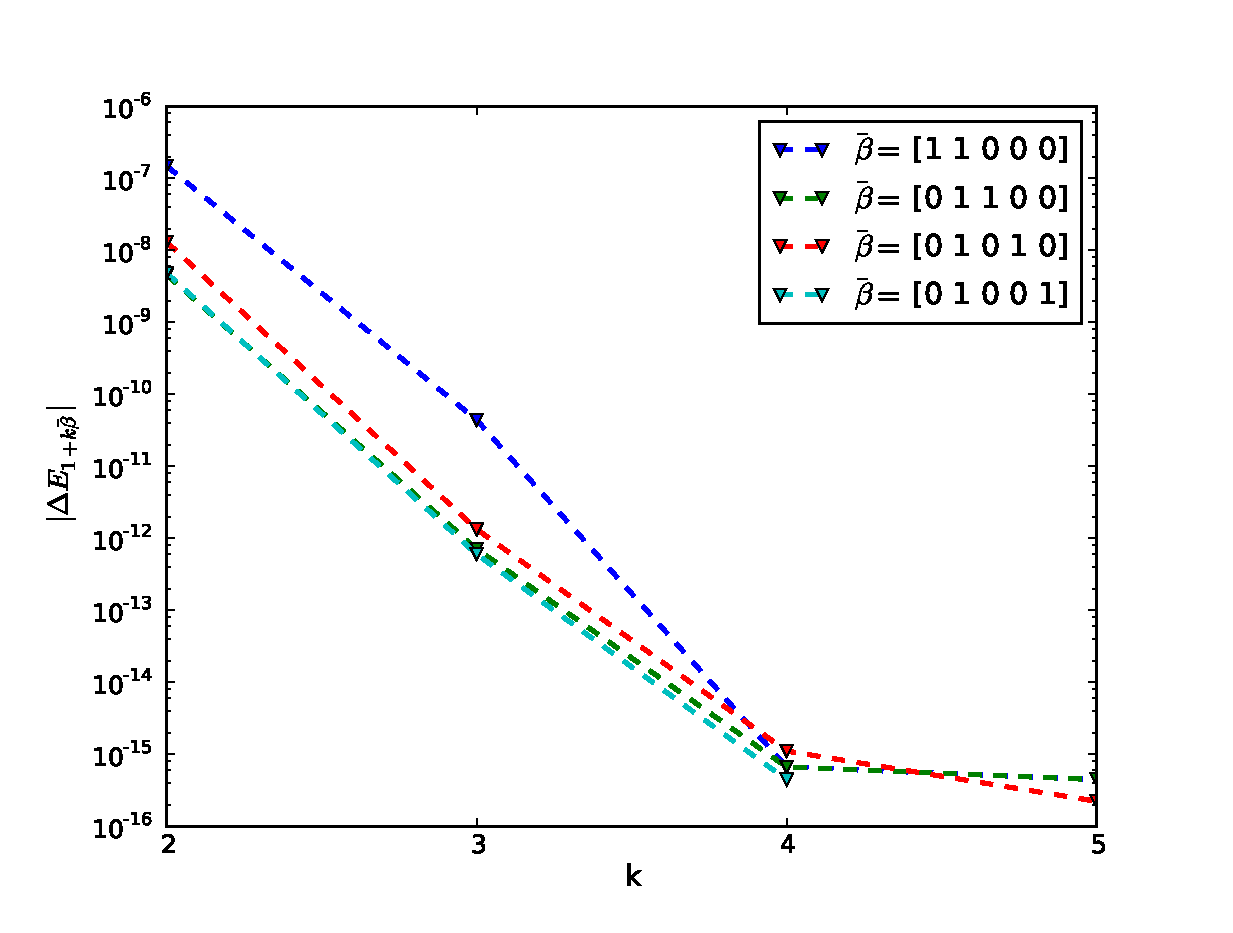
\includegraphics[width=1\linewidth]{./figures/mixed_difference_order2_basket_2.eps}
%		\caption{}
%		\label{fig:sub3}
%	\end{subfigure}%
%	\begin{subfigure}{.5\textwidth}
%		\centering
%		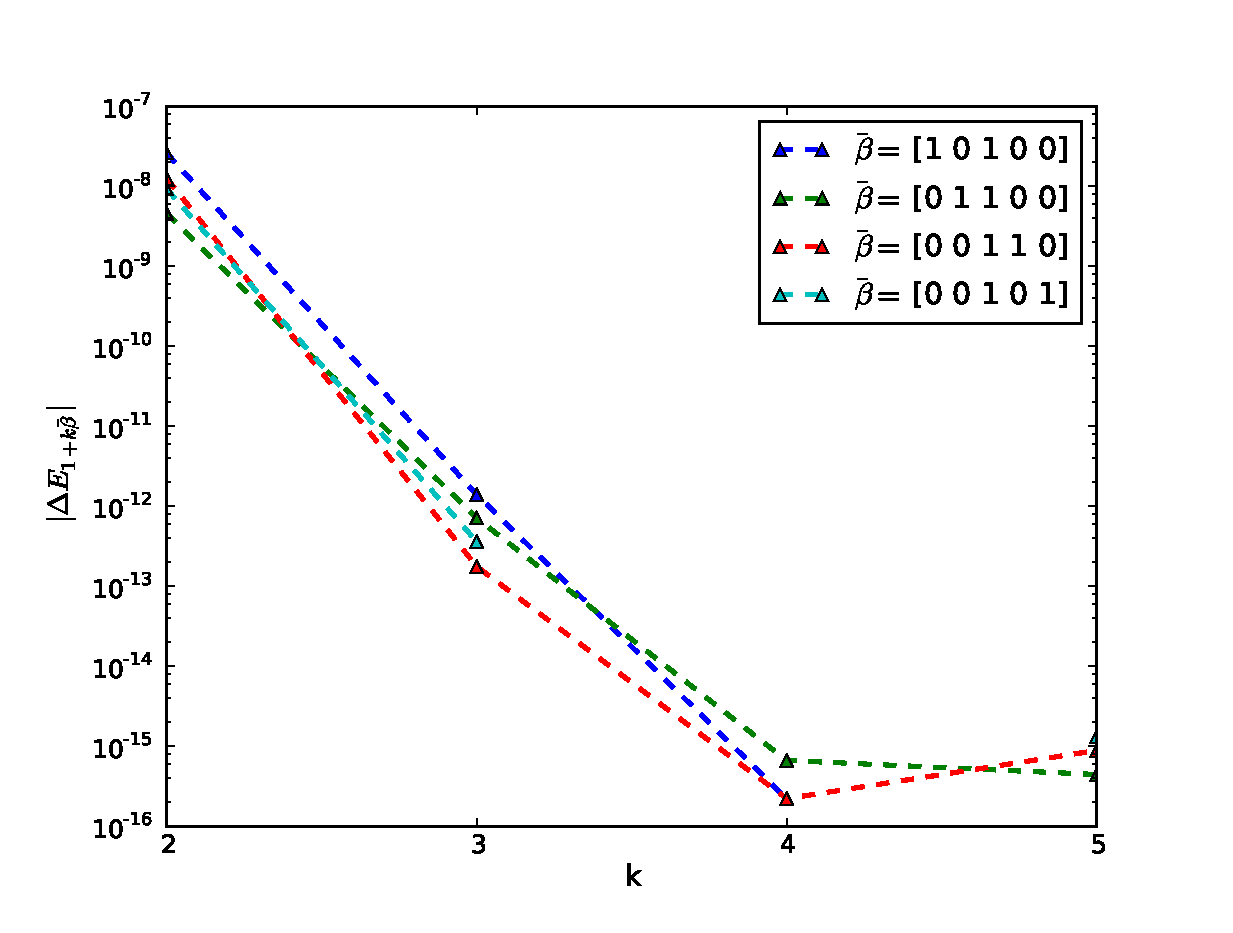
\includegraphics[width=1\linewidth]{./figures/mixed_difference_order2_basket_3.eps}
%		\caption{}
%		\label{fig:sub4}
%	\end{subfigure}
%
%	\caption{The rate of convergence of $\abs{\Delta E_{\beta}}$ ($\beta=\mathbf{1}+k \bar{\beta}$)): a) and b) show  the rate of convergence of second order mixed differences for different settings.}
%		\label{fig:test_basket_2}
%\end{figure}
%
%	\begin{figure}
%	\centering
%	\begin{subfigure}{.5\textwidth}
%		\centering
%		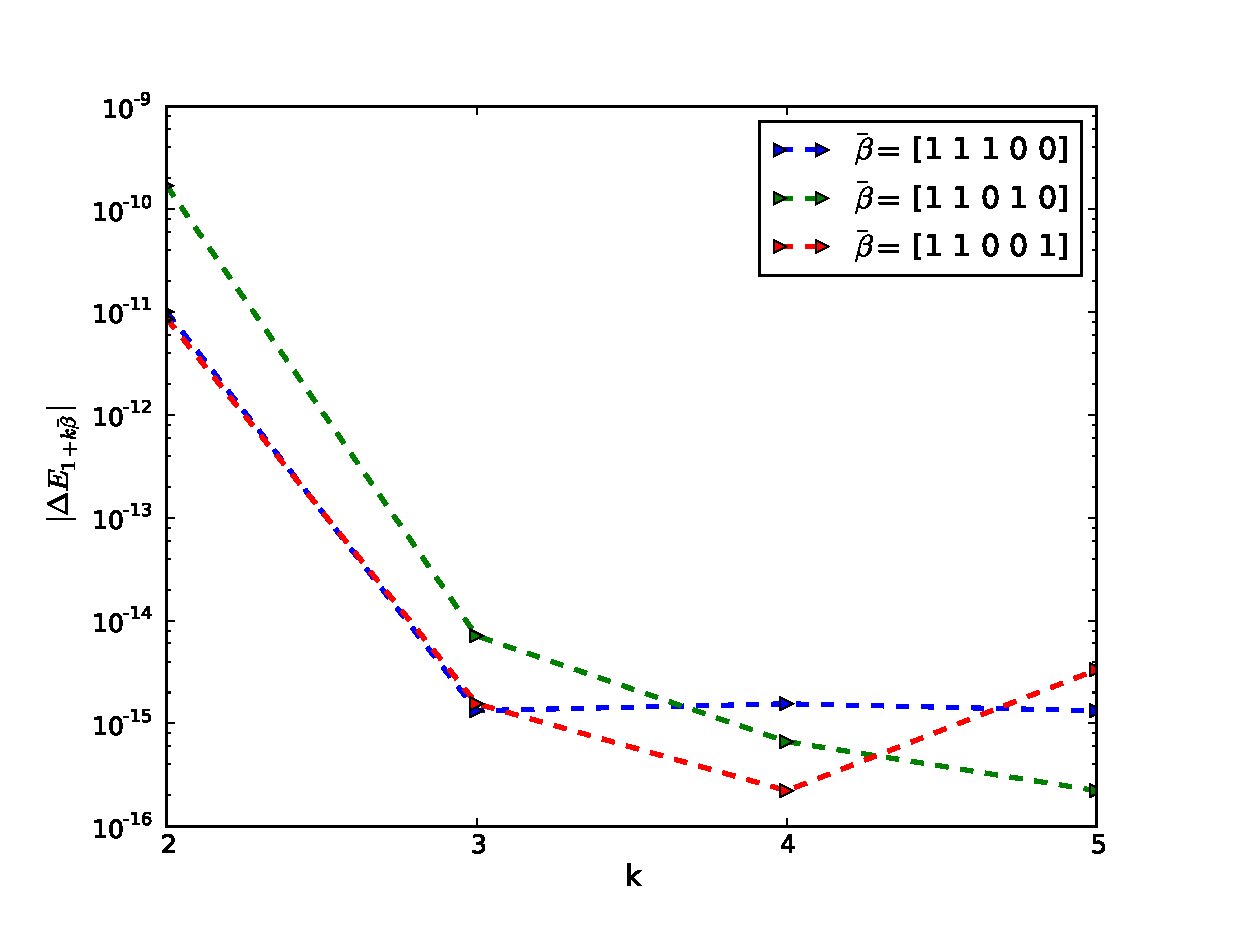
\includegraphics[width=1\linewidth]{./figures/mixed_difference_order3_basket_1.eps}
%	    \caption{}
%		\label{fig:sub5}
%	\end{subfigure}%
%	\begin{subfigure}{.5\textwidth}
%		\centering
%		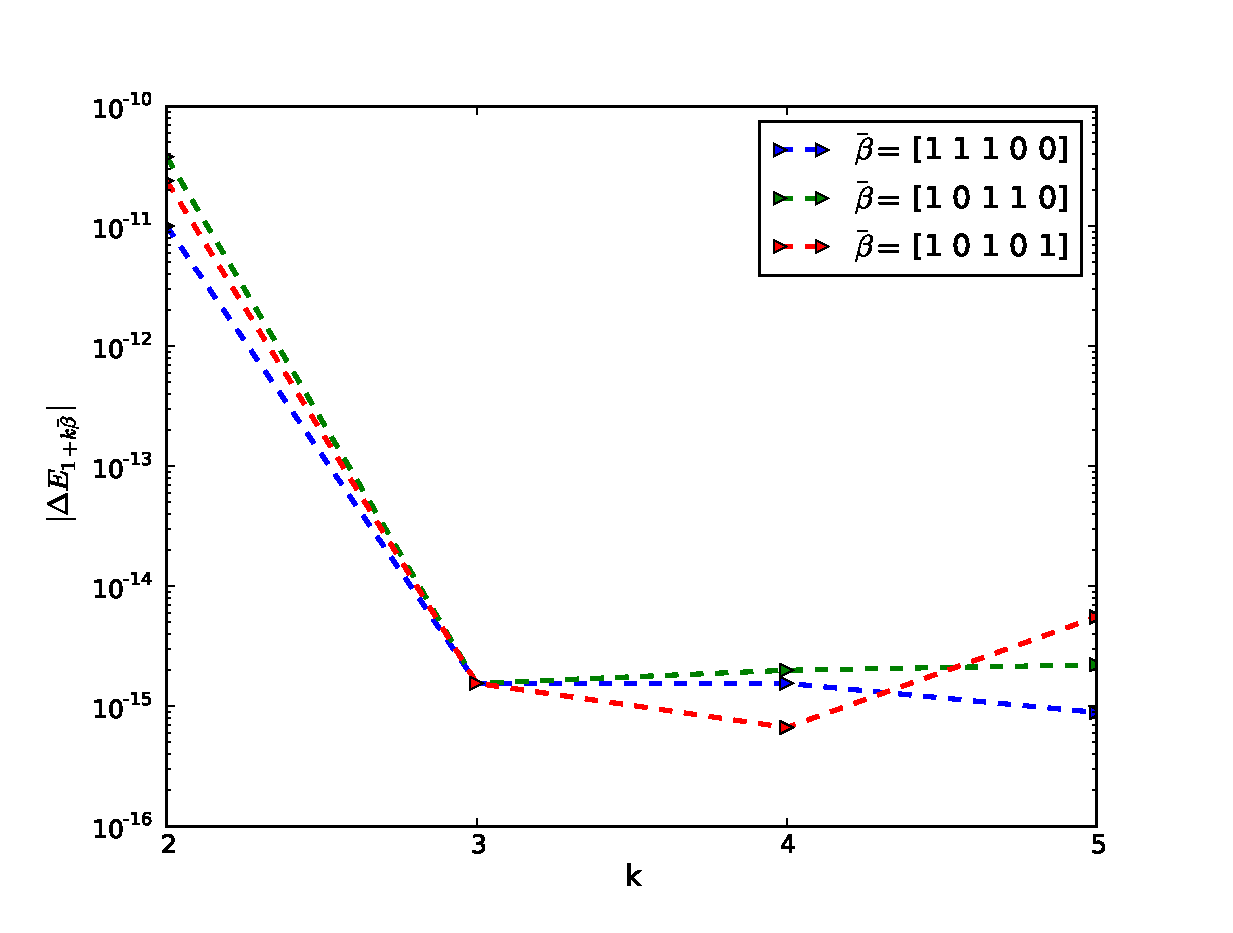
\includegraphics[width=1\linewidth]{./figures/mixed_difference_order3_basket_2.eps}
%		\caption{}
%		\label{fig:sub6}
%	\end{subfigure}
%	
%	\caption{The rate of convergence of $\abs{\Delta E_{\beta}}$ ($\beta=\mathbf{1}+k \bar{\beta}$): a) and b) show  the rate of convergence of third order mixed differences for different settings.}
%	\label{fig:test_basket_3}
%\end{figure}
%
%
%
% \newpage
%\section{Implementation details and  MISC results}\label{sec:Implementation details and  MISC results}
%The first step, when testing this example is to fix $\Delta t_{\text{min}}$ for the  time discretization parameter and do not introduce a hierarchy of levels in the deterministic dimension. Therefore, we will only construct a hierarchy of levels in the stochastic dimension associated with the Brownian increments. Then, the second step is to avoid this restriction of minimum  time discretization parameter (somehow like letting $\Delta t_{\text{min}} \rightarrow 0$)  and in that case, the problem will be close to do the integration in $\infty$-dimension, we need to see how the convergence rates will behave. The third step, is to use Richardson extrapolation which we expect bring the order of convergence for the Euler scheme from $ \ordo{\Delta t}$  to  $\ordo{\Delta t^2}$, and then we may expect that we will need fewer time steps to converge than the first case, and which means that fewer stochastic directions will be activated.   One technical difference here is that for $1$-dimensional, we will have two kink points instead of one but the procedure will be the same.  We note that we used Laguerre quadrature for integrating with respect to the dimension containing the kink. 
%
%Since we observed some problems for the results of the non-smooth payoff with Richardson extrapolation, we tried to add another case where we use a smoothed version of the call payoff to figure out the source of the problem. Using a smooth payoff allow us to separate the effect of infinite dimension and non-smoothness. As a possible choice, we use  the Black Scholes call option price formula, given by 
%\begin{equation}
%\mathrm C(\mathrm S,\mathrm t)= \mathrm N(\mathrm d_1)\mathrm S - \mathrm N(\mathrm d_2) \mathrm K \mathrm e^{-rt}
%\label{eq:2}
%\end{equation}
%
%\begin{equation}
%\mathrm d_1= \frac{1}{\sigma \sqrt{\mathrm t}} \left[\ln{\left(\frac{S}{K}\right)} + t\left(r + \frac{\sigma^2}{2} \right) \right]
%\end{equation}
%
%\begin{equation}
%\mathrm d_2= d_1- \sigma  \sqrt{t} 
%\end{equation}
%
%\begin{equation}
%N(x)=\frac{1}{\sqrt{2\pi}} \int_{-\infty}^{x} \mathrm e^{-\frac{1}{2}z^2} dz
%\label{eq:5}
%\end{equation}
%
%
%, which can be seen as a smoothed version of the true payoff (See figure \ref{fig:smooth_non_smooth}). The two differences with respect to the non-smooth case is that the dimension of the parameter space (stochastic space) now is increased by one  due to including the terminal value of the driving Brownian motion. Numerically, we observed weird results , in fact the quadrature performed worse than with the non-smooth case,  even for various values of volatilities. We still need to understand why this choice is not a good one. 
%
%
%Another possible choice that we worked with,  is by using the following smooth approximation of the max call payoff (See figure \ref{fig:smooth_payoff2})
%
%\begin{align}\label{eq:smooth_payoff2}
%	\operatorname{\max}_\epsilon(S-K,0) \approx 0.5 ( S-K+\sqrt{ (S-K)^{2}+\epsilon}),
%\end{align}
%
%where $\epsilon>0$.
%
%
%
%
%
%
%
%\begin{figure}[!h]
%	\centering
%	\begin{subfigure}{.5\textwidth}
%		\centering
%		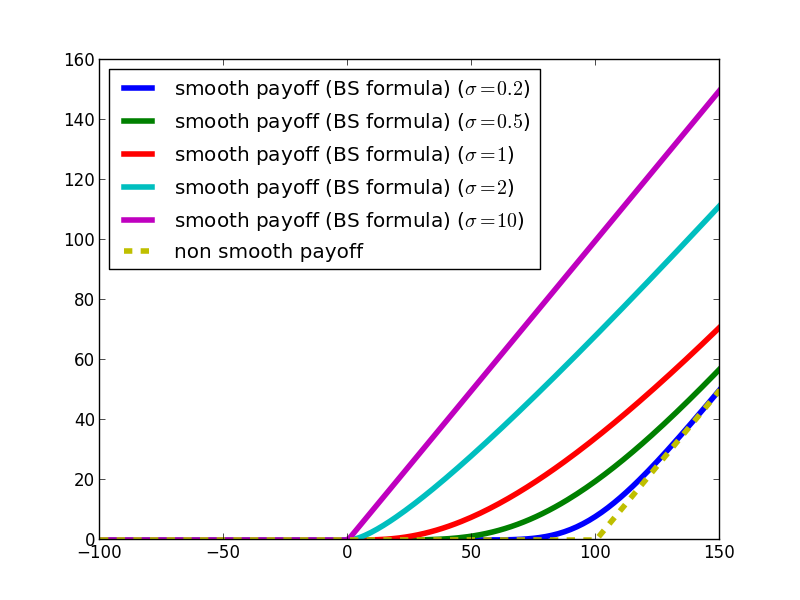
\includegraphics[width=1\linewidth]{./figures/smooth_non_smooth_payoff.png}
%		\caption{Black Scholes call option price for different values of $\sigma$}
%		\label{fig:smooth_non_smooth}
%	\end{subfigure}%
%	\begin{subfigure}{.5\textwidth}
%		\centering
%		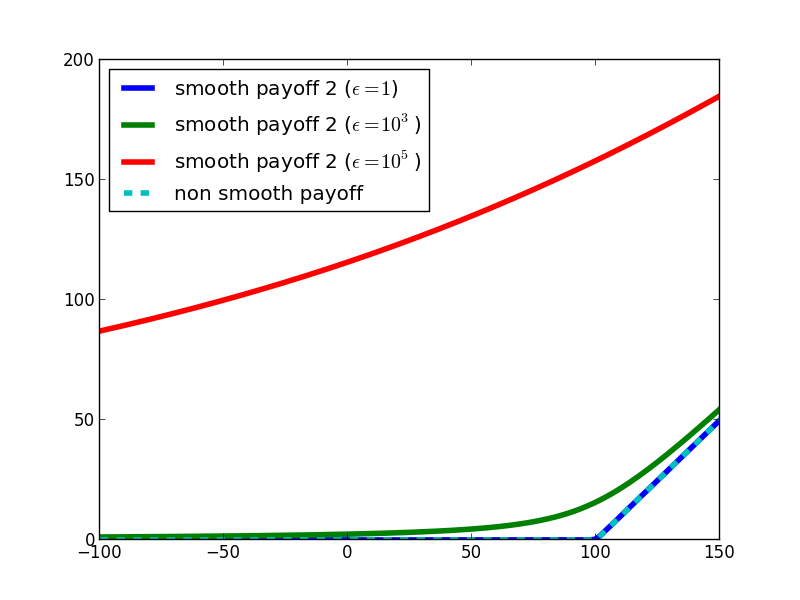
\includegraphics[width=1\linewidth]{./figures/smooth_payoff_2.png}
%		\caption{Smooth approximation of the max call payoff for different values of $\epsilon$.}
%		\label{fig:smooth_payoff2}
%	\end{subfigure}%
%\end{figure}
%
%
%
%%Numerically, we tried different values of $\epsilon$. For values of $\epsilon<10^5$, it is much expensive to run the quadrature compared to the non-smooth case( we need to understand why we have this behavior). 
%%In section \ref{sec:Results using MISC code_1D_BS}, we show some of the results with $8$ time steps and for $\epsilon=10^5$.
%%
%%\newpage
%%\subsubsection{A smooth payoff with Richardson extrapolation}
%%In this section, we present Richardson extrapolation algorithm that we use to compute the integrand before passing it to misc for the quadrature. We expect a slighter improvement of the rates  compared to cases without using Richardson extrapolation since $dt$ is fixed in the misc code (we assume that we do not have a deterministic direction, just stochastic ones). However, this improvement should be much better as $dt\rightarrow 0$ (higher number of time steps). In fact, since the convergence is fast with respect to the stochastic dimensions, the rate of convergence is deteriorated by the time-stepping procedure and then the advantage of using   Richardson extrapolation is to bring the order of convergence for the Euler scheme from $ \ordo{\Delta t}$  to  $\ordo{\Delta t^\alpha}$ ($\alpha>1$). This improvement implies that fewer stochastic directions will be activated and thus the improvement of the global rate of convergence.
%%
%%\begin{algorithm}
%%	\caption{Description of the Richardson algorithm }\label{euclid}
%%	\begin{algorithmic}[1]
%%%		\Procedure{MyProcedure}{}
%%		\State Initial set of quadrature points $y$, initial number of time steps $N$, $n:$ level of Richardson extrapolation, $\tilde{g}:$ the smooth payoff approximation
%%		\For{\texttt{$i=0$ to $n$}}
%%		\State $d_i0 \leftarrow \tilde{g}(\bar{X}_{N})$  ($\bar{X}_{N}$ is the stock price simulated with $N$ time steps and using $N$ quadrature points form $y$)
%%			\For{\texttt{$j=1$ to $i$}}
%%			\State $d_{i,j} \leftarrow d_{i,j-1}+(d_{i,j-1}-d_{i-1,j-1})/(4^j-1)$
%%			\EndFor
%%		\State $N \leftarrow 2 N	$
%%		\EndFor
%%		
%%		
%%		
%%%		\State $i \gets \textit{patlen}$
%%%		\BState \emph{top}:
%%%		\If {$i > \textit{stringlen}$} \Return false
%%%		\EndIf
%%%		\State $j \gets \textit{patlen}$
%%%		\BState \emph{loop}:
%%%		\If {$\textit{string}(i) = \textit{path}(j)$}
%%%		\State $j \gets j-1$.
%%%		\State $i \gets i-1$.
%%%		\State \textbf{goto} \emph{loop}.
%%%		\State \textbf{close};
%%%		\EndIf
%%%		\State $i \gets i+\max(\textit{delta}_1(\textit{string}(i)),\textit{delta}_2(j))$.
%%%		\State \textbf{goto} \emph{top}.
%%%		\EndProcedure
%%	\end{algorithmic}
%%\end{algorithm}
%%
%%
%%
%%
%
%
%%In the simulation, we  use consistent Brownian increments in simulating the paths of $\hat{X}^h$ and $\hat{X}^{2h}$, which results in a substantial reduction in variance. More specifically, each Brownian increment driving $\hat{X}^{2h}$ is the sum of two of the increments driving $\hat{X}^{h}$. This means that if we use $\sqrt{h} Z_1,\sqrt{h} Z_2,\dots $ as the Brownian increments for  $\hat{X}^{h}$ then we can use  $\sqrt{h} (Z_1+Z_2),\sqrt{h} (Z_3+Z_4),\dots $  as the Brownian increments for $\hat{X}^{2h}$.
%
%
%
%
%
%
%
%
%In table \ref{table: Complexity rates of the different methods for different number of time steps}, we summarize the results that we get in terms of complexity rates for different methods using different number of time steps. We clarify that the results for the Richardson extrapolation are given for just one level, where the associated steps in the table corresponds to those of level $1$.
%\begin{table}[h!]
%	\centering
%	\begin{tabular}{l*{6}{c}r}
%		Method \textbackslash  Steps            & $2$ & $4$ & $8$ & $16$  \\
%		\hline
%		Non-smooth payoff   & $-1/5$ & $-1/5$ & $-2/5$ & $-7/10$  \\
%		Non-smooth payoff with Richardson  extrapolation    & $-$ & $-$ & $-$ & $-$  \\
%		Smooth payoff(given by \eqref{eq:smooth_payoff2},$\epsilon=10^{-5}$)          & $-1/3$ &$-1/3$ &  $-3/5$ &  $-1$ \\
%		Smooth payoff with Richardson  extrapolation      & - & $-1/10$  & $-4/10$ & $-$  \\
%		\hline
%	\end{tabular}
%	\caption{Complexity rates of the different methods for different number of time steps}
%	\label{table: Complexity rates of the different methods for different number of time steps}
%\end{table}	
%
%Detailed plots for each case are given in appendix \ref{app: MISC Results 1D_BS}. Mainly, from the plots, 
%we checked  that we achive the prescribed tolerance using MISC, the convergence rates of mixed differences which is a basic assumption for using MISC (we observe exponential decay of error rates wrt to the number of quadrature points) and finally the complexity rates.
%
%\section{ MISC Results for the call option under discretized BS model}\label{app: MISC Results 1D_BS}
%
%\subsection{Case of $2$ time steps with non-smooth payoff}
%
%From the following plots, we confirm the exponential rate of convergence for the stochastic parameters, we achieve the prescribed tolerance and  we get a rate of complexity (in terms of average running time) approximately of order $-1/5$ for $2$ time steps.
%\begin{figure}[!h]
%	\centering
%	\begin{subfigure}{.5\textwidth}
%		\centering
%		\includegraphics[width=1\linewidth]{./figures/1D_BS_2_steps_non_smooth/error_estimate.pdf}
%		\caption{Error estimate}
%		\label{fig:misc_1D_BS_non_smooth_2steps_sub1}
%	\end{subfigure}%
%	\begin{subfigure}{.5\textwidth}
%		\centering
%		\includegraphics[width=1\linewidth]{./figures/1D_BS_2_steps_non_smooth/average_running_time.pdf}
%		\caption{Average running time as a function of $TOL$}
%		\label{fig:misc_1D_BS_non_smooth_2steps_sub2}
%	\end{subfigure}%
%	\caption{Convergence and complexity results for for the $1D$ BS model with the non-smooth call payoff.}
%	\label{fig:misc_1D_BS_nonsmooth_2steps_2}
%\end{figure}
%
%
%
%\begin{figure}[!h]
%	\centering
%	\begin{subfigure}{.5\textwidth}
%		\centering
%		\includegraphics[width=0.95\linewidth]{./figures/1D_BS_2_steps_non_smooth/level_work.pdf}
%		\caption{Average Computational time per level}
%		\label{fig:misc_1D_BS_non_smooth_2steps_sub3}
%	\end{subfigure}%
%	\begin{subfigure}{.5\textwidth}
%		\centering
%		\includegraphics[width=0.95\linewidth]{./figures/1D_BS_2_steps_non_smooth/levels_error_rate.pdf}
%		\caption{ The convergence rate of first differences per level}
%		\label{fig:misc_1D_BS_non_smooth_2steps_sub4}
%	\end{subfigure}%
%	\caption{Convergence and work rates for discretization levels for the $1D$ BS model with the non-smooth call payoff.}
%	\label{fig:misc_1D_BS_2teps_2}
%\end{figure}
%
%
%
%\subsection{Case of $2$ time steps with smooth payoff (given by \eqref{eq:smooth_payoff2})}
%
%From the following plots, we confirm the exponential rate of convergence for the stochastic parameters, we achieve the prescribed tolerance and  we get a rate of complexity (in terms of average running time) approximately of order $-1/3$ for $2$ time steps.
%
%\begin{figure}[!h]
%	\centering
%	\begin{subfigure}{.5\textwidth}
%		\centering
%		\includegraphics[width=1\linewidth]{./figures/1D_BS_2_steps_smooth_second_payoff_eps_10_5/error_estimate.pdf}
%		\caption{Error estimate}
%		\label{fig:misc_1D_BS_2_steps_smooth_second_payoff_eps_10_5_sub1}
%	\end{subfigure}%
%	\begin{subfigure}{.5\textwidth}
%		\centering
%		\includegraphics[width=1\linewidth]{./figures/1D_BS_2_steps_smooth_second_payoff_eps_10_5/average_running_time.pdf}
%		\caption{Average running time as a function of $TOL$}
%		\label{fig:misc_1D_BS_2_steps_smooth_second_payoff_eps_10_5_sub2}
%	\end{subfigure}%
%	\caption{Convergence and complexity results for for the $1D$ BS model with the smooth call payoff given by \eqref{eq:smooth_payoff2}.}
%	\label{fig:misc_1D_BS_2_steps_smooth_second_payoff_eps_10_5_1}
%\end{figure}
%
%
%
%\begin{figure}[!h]
%	\centering
%	\begin{subfigure}{.5\textwidth}
%		\centering
%		\includegraphics[width=0.95\linewidth]{./figures/1D_BS_2_steps_smooth_second_payoff_eps_10_5/level_work.pdf}
%		\caption{Average Computational time per level}
%		\label{fig:misc_1D_BS_2_steps_smooth_second_payoff_eps_10_5_sub3}
%	\end{subfigure}%
%	\begin{subfigure}{.5\textwidth}
%		\centering
%		\includegraphics[width=0.95\linewidth]{./figures/1D_BS_2_steps_smooth_second_payoff_eps_10_5/levels_error_rate.pdf}
%		\caption{ The convergence rate of first differences per level}
%		\label{fig:misc_1D_BS_2_steps_smooth_second_payoff_eps_10_5_sub4}
%	\end{subfigure}%
%	\caption{Convergence and work rates for discretization levels for the $1D$ BS model with the smooth call payoff given by \eqref{eq:smooth_payoff2}.}
%	\label{fig:misc_1D_BS_2_steps_smooth_second_payoff_eps_10_5_2}
%\end{figure}
%
%
%\newpage
%
%
%
%
%\subsection{Case of $4$ time steps with non-smooth payoff}
%
%From the following plots, we confirm the exponential rate of convergence for the stochastic parameters, we achieve the prescribed tolerance and  we get a rate of complexity (in terms of average running time) approximately of order $-1/5$ for $4$ time steps.
%\begin{figure}[!h]
%	\centering
%	\begin{subfigure}{.5\textwidth}
%		\centering
%		\includegraphics[width=1\linewidth]{./figures/1D_BS_4_steps_non_smooth/error_estimate.pdf}
%		\caption{Error estimate}
%		\label{fig:misc_1D_BS_non_smooth_4steps_sub1}
%	\end{subfigure}%
%	\begin{subfigure}{.5\textwidth}
%		\centering
%		\includegraphics[width=1\linewidth]{./figures/1D_BS_4_steps_non_smooth/average_running_time.pdf}
%		\caption{Average running time as a function of $TOL$}
%		\label{fig:misc_1D_BS_non_smooth_4steps_sub2}
%	\end{subfigure}%
%	\caption{Convergence and complexity results for for the $1D$ BS model with the non-smooth call payoff .}
%	\label{fig:misc_1D_BS_nonsmooth_4steps_2}
%\end{figure}
%
%
%
%\begin{figure}[!h]
%	\centering
%	\begin{subfigure}{.5\textwidth}
%		\centering
%		\includegraphics[width=0.95\linewidth]{./figures/1D_BS_4_steps_non_smooth/level_work.pdf}
%		\caption{Average Computational time per level}
%		\label{fig:misc_1D_BS_non_smooth_4steps_sub3}
%	\end{subfigure}%
%	\begin{subfigure}{.5\textwidth}
%		\centering
%		\includegraphics[width=0.95\linewidth]{./figures/1D_BS_4_steps_non_smooth/levels_error_rate.pdf}
%		\caption{ The convergence rate of first differences per level}
%		\label{fig:misc_1D_BS_non_smooth_4steps_sub4}
%	\end{subfigure}%
%	\caption{Convergence and work rates for discretization levels for the $1D$ BS model with the non- smooth call payoff.}
%	\label{fig:misc_1D_BS_4teps_2}
%\end{figure}
%
%
%\newpage
%
%\subsection{Case of non smooth payoff  with Richardson extrapolation (level $0$: $2$ time steps, level $1$: $4$ time steps) (Ignoring the middle part of integration)}
%
%From the following plots, we confirm the exponential rate of convergence for the stochastic parameters, we achieve the prescribed tolerance and  we get a rate of complexity (in terms of average running time) approximately of order $-1/2$.
%
%\begin{figure}[!h]
%	\centering
%	\begin{subfigure}{.5\textwidth}
%		\centering
%		\includegraphics[width=1\linewidth]{./figures/1D_BS_2_4_step_non_smooth_richardson_without_middle/error_estimate.pdf}
%		\caption{Error estimate}
%		\label{fig:misc_1D_BS_2_4_step_non_smooth_richardson_without_middle_sub1}
%	\end{subfigure}%
%	\begin{subfigure}{.5\textwidth}
%		\centering
%		\includegraphics[width=1\linewidth]{./figures/1D_BS_2_4_step_non_smooth_richardson_without_middle/average_running_time.pdf}
%		\caption{Average running time as a function of $TOL$}
%		\label{fig:misc_1D_BS_2_4_step_non_smooth_richardson_without_middle_sub2}
%	\end{subfigure}%
%	\caption{Convergence and complexity results for for the $1D$ BS model with the non smooth call payoff with Richardson extrapolation (Ignoring the middle part of integration).}
%	\label{fig:misc_1D_BS_2_4_step_non_smooth_richardson_without_middle_1}
%\end{figure}
%
%
%
%\begin{figure}[!h]
%	\centering
%	\begin{subfigure}{.5\textwidth}
%		\centering
%		\includegraphics[width=0.95\linewidth]{./figures/1D_BS_2_4_step_non_smooth_richardson_without_middle/level_work.pdf}
%		\caption{Average Computational time per level}
%		\label{fig:misc_1D_BS_2_4_step_non_smooth_richardson_without_middle_sub3}
%	\end{subfigure}%
%	\begin{subfigure}{.5\textwidth}
%		\centering
%		\includegraphics[width=0.95\linewidth]{./figures/1D_BS_2_4_step_non_smooth_richardson_without_middle/levels_error_rate.pdf}
%		\caption{ The convergence rate of first differences per level}
%		\label{fig:misc_1D_BS_2_4_step_non_smooth_richardson_without_middle_sub4}
%	\end{subfigure}%
%	\caption{Convergence and work rates for discretization levels for the $1D$ BS model with the non smooth call payoff with Richardson extrapolation (Ignoring the middle part of integration).}
%	\label{fig:misc_1D_BS_2_4_step_non_smooth_richardson_without_middle_2}
%\end{figure}
%\newpage
%
%
%\subsection{Case of $4$ time steps with smooth payoff (given by \eqref{eq:smooth_payoff2})}
%
%From the following plots, we confirm the exponential rate of convergence for the stochastic parameters, we achieve the prescribed tolerance and  we get a rate of complexity (in terms of average running time) approximately of order $-1/3$ for $4$ time steps.
%
%\begin{figure}[!h]
%	\centering
%	\begin{subfigure}{.5\textwidth}
%		\centering
%		\includegraphics[width=1\linewidth]{./figures/1D_BS_4_steps_smooth_second_payoff_eps_10_5/error_estimate.pdf}
%		\caption{Error estimate}
%		\label{fig:misc_1D_BS_4_steps_smooth_second_payoff_eps_10_5_sub1}
%	\end{subfigure}%
%	\begin{subfigure}{.5\textwidth}
%		\centering
%		\includegraphics[width=1\linewidth]{./figures/1D_BS_4_steps_smooth_second_payoff_eps_10_5/average_running_time.pdf}
%		\caption{Average running time as a function of $TOL$}
%		\label{fig:misc_1D_BS_4_steps_smooth_second_payoff_eps_10_5_sub2}
%	\end{subfigure}%
%	\caption{Convergence and complexity results for for the $1D$ BS model with the smooth call payoff given by \eqref{eq:smooth_payoff2}.}
%	\label{fig:misc_1D_BS_4_steps_smooth_second_payoff_eps_10_5_1}
%\end{figure}
%
%
%
%\begin{figure}[!h]
%	\centering
%	\begin{subfigure}{.5\textwidth}
%		\centering
%		\includegraphics[width=0.95\linewidth]{./figures/1D_BS_4_steps_smooth_second_payoff_eps_10_5/level_work.pdf}
%		\caption{Average Computational time per level}
%		\label{fig:misc_1D_BS_4_steps_smooth_second_payoff_eps_10_5_sub3}
%	\end{subfigure}%
%	\begin{subfigure}{.5\textwidth}
%		\centering
%		\includegraphics[width=0.95\linewidth]{./figures/1D_BS_4_steps_smooth_second_payoff_eps_10_5/levels_error_rate.pdf}
%		\caption{ The convergence rate of first differences per level}
%		\label{fig:misc_1D_BS_4_steps_smooth_second_payoff_eps_10_5_sub4}
%	\end{subfigure}%
%	\caption{Convergence and work rates for discretization levels for the $1D$ BS model with the smooth call payoff given by \eqref{eq:smooth_payoff2}.}
%	\label{fig:misc_1D_BS_4_steps_smooth_second_payoff_eps_10_5_2}
%\end{figure}
%
%\newpage
%
%
%
%
%
%\subsection{Case of smooth payoff (given by \eqref{eq:smooth_payoff2}) with Richardson extrapolation (level $0$: $2$ time steps, level $1$: $4$ time steps)}
%From the following plots, we confirm the exponential rate of convergence for the stochastic parameters, we achieve the prescribed tolerance and  we get a rate of complexity (in terms of average running time) approximately of order $-1/10$.
%
%\begin{figure}[!h]
%	\centering
%	\begin{subfigure}{.5\textwidth}
%		\centering
%		\includegraphics[width=1\linewidth]{./figures/1D_BS_2_4_steps_smooth_second_payoff_eps_10_5_richardson/error_estimate.pdf}
%		\caption{Error estimate}
%		\label{fig:misc_1D_BS_2_4_steps_smooth_second_payoff_eps_10_5_sub1}
%	\end{subfigure}%
%	\begin{subfigure}{.5\textwidth}
%		\centering
%		\includegraphics[width=1\linewidth]{./figures/1D_BS_2_4_steps_smooth_second_payoff_eps_10_5_richardson/average_running_time.pdf}
%		\caption{Average running time as a function of $TOL$}
%		\label{fig:misc_1D_BS_2_4_steps_smooth_second_payoff_eps_10_5_sub2}
%	\end{subfigure}%
%	\caption{Convergence and complexity results for for the $1D$ BS model with the smooth call payoff given by \eqref{eq:smooth_payoff2} with Richardson extrapolation.}
%	\label{fig:misc_1D_BS_2_4_steps_smooth_second_payoff_eps_10_5_1}
%\end{figure}
%
%
%
%\begin{figure}[!h]
%	\centering
%	\begin{subfigure}{.5\textwidth}
%		\centering
%		\includegraphics[width=0.95\linewidth]{./figures/1D_BS_4_8_steps_smooth_second_payoff_eps_10_5_richardson/level_work.pdf}
%		\caption{Average Computational time per level}
%		\label{fig:misc_1D_BS_2_4_steps_smooth_second_payoff_eps_10_sub3}
%	\end{subfigure}%
%	\begin{subfigure}{.5\textwidth}
%		\centering
%		\includegraphics[width=0.95\linewidth]{./figures/1D_BS_2_4_steps_smooth_second_payoff_eps_10_5_richardson/levels_error_rate.pdf}
%		\caption{ The convergence rate of first differences per level}
%		\label{fig:misc_1D_BS_2_4_steps_smooth_second_payoff_eps_10_5_sub4}
%	\end{subfigure}%
%	\caption{Convergence and work rates for discretization levels for the $1D$ BS model with the smooth call payoff given by \eqref{eq:smooth_payoff2} with Richardson extrapolation.}
%	\label{fig:misc_1D_BS_2_4_steps_smooth_second_payoff_eps_10_5_2}
%\end{figure}
%\newpage
%
%
%\subsection{Case of $8$ time steps with non-smooth payoff}
%
%From the following plots, we confirm the exponential rate of convergence for the stochastic parameters, we achieve the prescribed tolerance and  we get a rate of complexity (in terms of average running time) approximately of order $-2/5$ for $8$ time steps.
%\begin{figure}[!h]
%	\centering
%	\begin{subfigure}{.5\textwidth}
%		\centering
%		\includegraphics[width=1\linewidth]{./figures/1D_BS_8_steps_non_smooth/error_estimate.pdf}
%		\caption{Error estimate}
%		\label{fig:misc_1D_BS_non_smooth_8steps_sub1}
%	\end{subfigure}%
%	\begin{subfigure}{.5\textwidth}
%		\centering
%		\includegraphics[width=1\linewidth]{./figures/1D_BS_8_steps_non_smooth/average_running_time.pdf}
%		\caption{Average running time as a function of $TOL$}
%		\label{fig:misc_1D_BS_non_smooth_8steps_sub2}
%	\end{subfigure}%
%	\caption{Convergence and complexity results for for the $1D$ BS model with the non-smooth call payoff.}
%	\label{fig:misc_1D_BS_nonsmooth_8steps_2}
%\end{figure}
%
%
%
%\begin{figure}[!h]
%	\centering
%	\begin{subfigure}{.5\textwidth}
%		\centering
%		\includegraphics[width=0.95\linewidth]{./figures/1D_BS_8_steps_non_smooth/level_work.pdf}
%		\caption{Average Computational time per level}
%		\label{fig:misc_1D_BS_non_smooth_8steps_sub3}
%	\end{subfigure}%
%	\begin{subfigure}{.5\textwidth}
%		\centering
%		\includegraphics[width=0.95\linewidth]{./figures/1D_BS_8_steps_non_smooth/levels_error_rate.pdf}
%		\caption{ The convergence rate of first differences per level}
%		\label{fig:misc_1D_BS_non_smooth_8steps_sub4}
%	\end{subfigure}%
%	\caption{Convergence and work rates for discretization levels for the $1D$ BS model with the non- smooth call payoff.}
%	\label{fig:misc_1D_BS_8teps_2}
%\end{figure}
%
%% \newpage
%%\subsubsection*{Case of $8$ time steps with smooth payoff (BS formula)}
%%
%%
%%
%%\begin{figure}[!h]
%%	\centering
%%	\begin{subfigure}{.5\textwidth}
%%		\centering
%%		\includegraphics[width=1\linewidth]{./figures/1D_BS_8_steps_smooth_BS_payoff/error_estimate.pdf}
%%		\caption{}
%%		\label{fig:misc_1D_BS_8_steps_smooth_BS_payoff_sub1}
%%	\end{subfigure}%
%%	\begin{subfigure}{.5\textwidth}
%%		\centering
%%		\includegraphics[width=1\linewidth]{./figures/1D_BS_8_steps_smooth_BS_payoff/average_running_time.pdf}
%%		\caption{}
%%		\label{fig:misc_1D_BS_8_steps_smooth_BS_payoff_sub2}
%%	\end{subfigure}%
%%	\caption{.}
%%	\label{fig:misc_1D_BS_8_steps_smooth_BS_payoff_1}
%%\end{figure}
%%
%%
%%
%%\begin{figure}[!h]
%%	\centering
%%	\begin{subfigure}{.5\textwidth}
%%		\centering
%%		\includegraphics[width=0.95\linewidth]{./figures/1D_BS_8_steps_smooth_BS_payoff/level_work.pdf}
%%		\caption{}
%%		\label{fig:misc_1D_BS_8_steps_smooth_BS_payoff_sub3}
%%	\end{subfigure}%
%%	\begin{subfigure}{.5\textwidth}
%%		\centering
%%		\includegraphics[width=0.95\linewidth]{./figures/1D_BS_8_steps_smooth_BS_payoff/levels_error_rate.pdf}
%%		\caption{}
%%		\label{fig:misc_1D_BS_8_steps_smooth_BS_payoff_sub4}
%%	\end{subfigure}%
%%	\caption{.}
%%	\label{fig:misc_1D_BS_8_steps_smooth_BS_payoff_2}
%%\end{figure}
%\newpage
%
%\subsection{Case of non smooth payoff  with Richardson extrapolation (level $0$: $4$ time steps, level $1$: $8$ time steps) (Ignoring the middle part of integration)}
%
%From the following plots, we confirm the exponential rate of convergence for the stochastic parameters, we achieve the prescribed tolerance and  we get a rate of complexity (in terms of average running time) approximately of order $-1/2$.
%
%\begin{figure}[!h]
%	\centering
%	\begin{subfigure}{.5\textwidth}
%		\centering
%		\includegraphics[width=1\linewidth]{./figures/1D_BS_4_8_step_non_smooth_richardson_without_middle/error_estimate.pdf}
%		\caption{Error estimate}
%		\label{fig:misc_1D_BS_4_8_step_non_smooth_richardson_without_middle_sub1}
%	\end{subfigure}%
%	\begin{subfigure}{.5\textwidth}
%		\centering
%		\includegraphics[width=1\linewidth]{./figures/1D_BS_4_8_step_non_smooth_richardson_without_middle/average_running_time.pdf}
%		\caption{Average running time as a function of $TOL$}
%		\label{fig:misc_1D_BS_4_8_step_non_smooth_richardson_without_middle_sub2}
%	\end{subfigure}%
%	\caption{Convergence and complexity results for for the $1D$ BS model with the non smooth call payoff with Richardson extrapolation (Ignoring the middle part of integration).}
%	\label{fig:misc_1D_BS_4_8_step_non_smooth_richardson_without_middle_1}
%\end{figure}
%
%
%
%\begin{figure}[!h]
%	\centering
%	\begin{subfigure}{.5\textwidth}
%		\centering
%		\includegraphics[width=0.95\linewidth]{./figures/1D_BS_4_8_step_non_smooth_richardson_without_middle/level_work.pdf}
%		\caption{Average Computational time per level}
%		\label{fig:misc_1D_BS_4_8_step_non_smooth_richardson_without_middle_sub3}
%	\end{subfigure}%
%	\begin{subfigure}{.5\textwidth}
%		\centering
%		\includegraphics[width=0.95\linewidth]{./figures/1D_BS_4_8_step_non_smooth_richardson_without_middle/levels_error_rate.pdf}
%		\caption{ The convergence rate of first differences per level}
%		\label{fig:misc_1D_BS_4_8_step_non_smooth_richardson_without_middle_sub4}
%	\end{subfigure}%
%	\caption{Convergence and work rates for discretization levels for the $1D$ BS model with the non smooth call payoff with Richardson extrapolation (Ignoring the middle part of integration).}
%	\label{fig:misc_1D_BS_4_8_step_non_smooth_richardson_without_middle_2}
%\end{figure}
%\newpage
%
%
%\subsection{Case of $8$ time steps with smooth payoff (given by \eqref{eq:smooth_payoff2})}
%
%From the following plots, we confirm the exponential rate of convergence for the stochastic parameters, we achieve the prescribed tolerance and  we get a rate of complexity (in terms of average running time) approximately of order $-3/5$ for $8$ time steps.
%
%\begin{figure}[!h]
%	\centering
%	\begin{subfigure}{.5\textwidth}
%		\centering
%		\includegraphics[width=1\linewidth]{./figures/1D_BS_8_steps_smooth_second_payoff_eps_10_5/error_estimate.pdf}
%		\caption{Error estimate}
%		\label{fig:misc_1D_BS_8_steps_smooth_second_payoff_eps_10_5_sub1}
%	\end{subfigure}%
%	\begin{subfigure}{.5\textwidth}
%		\centering
%		\includegraphics[width=1\linewidth]{./figures/1D_BS_8_steps_smooth_second_payoff_eps_10_5/average_running_time.pdf}
%		\caption{Average running time as a function of $TOL$}
%		\label{fig:misc_1D_BS_8_steps_smooth_second_payoff_eps_10_5_sub2}
%	\end{subfigure}%
%	\caption{Convergence and complexity results for for the $1D$ BS model with the smooth call payoff given by \eqref{eq:smooth_payoff2}.}
%	\label{fig:misc_1D_BS_8_steps_smooth_second_payoff_eps_10_5_1}
%\end{figure}
%
%
%
%\begin{figure}[!h]
%	\centering
%	\begin{subfigure}{.5\textwidth}
%		\centering
%		\includegraphics[width=0.95\linewidth]{./figures/1D_BS_8_steps_smooth_second_payoff_eps_10_5/level_work.pdf}
%		\caption{Average Computational time per level}
%		\label{fig:misc_1D_BS_8_steps_smooth_second_payoff_eps_10_5_sub3}
%	\end{subfigure}%
%	\begin{subfigure}{.5\textwidth}
%		\centering
%		\includegraphics[width=0.95\linewidth]{./figures/1D_BS_8_steps_smooth_second_payoff_eps_10_5/levels_error_rate.pdf}
%		\caption{ The convergence rate of first differences per level}
%		\label{fig:misc_1D_BS_8_steps_smooth_second_payoff_eps_10_5_sub4}
%	\end{subfigure}%
%	\caption{Convergence and work rates for discretization levels for the $1D$ BS model with the smooth call payoff given by \eqref{eq:smooth_payoff2}.}
%	\label{fig:misc_1D_BS_8_steps_smooth_second_payoff_eps_10_5_2}
%\end{figure}
%
%
%\newpage
%
%
%\subsection{Case of smooth payoff (given by \eqref{eq:smooth_payoff2}) with Richardson extrapolation (level $0$: $4$ time steps, level $1$: $8$ time steps)}
%From the following plots, we confirm the exponential rate of convergence for the stochastic parameters, we achieve the prescribed tolerance and  we get a rate of complexity (in terms of average running time) approximately of order $-4/10$.
%
%\begin{figure}[!h]
%	\centering
%	\begin{subfigure}{.5\textwidth}
%		\centering
%		\includegraphics[width=1\linewidth]{./figures/1D_BS_4_8_steps_smooth_second_payoff_eps_10_5_richardson/error_estimate.pdf}
%		\caption{Error estimate}
%		\label{fig:misc_1D_BS_4_8_steps_smooth_second_payoff_eps_10_5_sub1}
%	\end{subfigure}%
%	\begin{subfigure}{.5\textwidth}
%		\centering
%		\includegraphics[width=1\linewidth]{./figures/1D_BS_4_8_steps_smooth_second_payoff_eps_10_5_richardson/average_running_time.pdf}
%		\caption{Average running time as a function of $TOL$}
%		\label{fig:misc_1D_BS_4_8_steps_smooth_second_payoff_eps_10_5_sub2}
%	\end{subfigure}%
%	\caption{Convergence and complexity results for for the $1D$ BS model with the smooth call payoff given by \eqref{eq:smooth_payoff2} with Richardson extrapolation.}
%	\label{fig:misc_1D_BS_4_8_steps_smooth_second_payoff_eps_10_5_1}
%\end{figure}
%
%
%
%\begin{figure}[!h]
%	\centering
%	\begin{subfigure}{.5\textwidth}
%		\centering
%		\includegraphics[width=0.95\linewidth]{./figures/1D_BS_4_8_steps_smooth_second_payoff_eps_10_5_richardson/level_work.pdf}
%		\caption{Average Computational time per level}
%		\label{fig:misc_1D_BS_4_8_steps_smooth_second_payoff_eps_10_sub3}
%	\end{subfigure}%
%	\begin{subfigure}{.5\textwidth}
%		\centering
%		\includegraphics[width=0.95\linewidth]{./figures/1D_BS_4_8_steps_smooth_second_payoff_eps_10_5_richardson/levels_error_rate.pdf}
%		\caption{ The convergence rate of first differences per level}
%		\label{fig:misc_1D_BS_4_8_steps_smooth_second_payoff_eps_10_5_sub4}
%	\end{subfigure}%
%	\caption{Convergence and work rates for discretization levels for the $1D$ BS model with the smooth call payoff given by \eqref{eq:smooth_payoff2} with Richardson extrapolation.}
%	\label{fig:misc_1D_BS_4_8_steps_smooth_second_payoff_eps_10_5_2}
%\end{figure}
%
%\newpage
%\subsection{Case of $16$ time steps with non-smooth payoff}
%
%From the following plots, we confirm the exponential rate of convergence for the stochastic parameters, we achieve the prescribed tolerance and  we get a rate of complexity (in terms of average running time) approximately of order $-7/10$ for $16$ time steps.
%\begin{figure}[!h]
%	\centering
%	\begin{subfigure}{.5\textwidth}
%		\centering
%		\includegraphics[width=1\linewidth]{./figures/1D_BS_16_steps_non_smooth/error_estimate.pdf}
%		\caption{Error estimate}
%		\label{fig:misc_1D_BS_non_smooth_16steps_sub1}
%	\end{subfigure}%
%	\begin{subfigure}{.5\textwidth}
%		\centering
%		\includegraphics[width=1\linewidth]{./figures/1D_BS_16_steps_non_smooth/average_running_time.pdf}
%		\caption{Average running time as a function of $TOL$}
%		\label{fig:misc_1D_BS_non_smooth_816steps_sub2}
%	\end{subfigure}%
%	\caption{Convergence and complexity results for for the $1D$ BS model with the non-smooth call payoff.}
%	\label{fig:misc_1D_BS_nonsmooth_16steps_2}
%\end{figure}
%
%
%
%\begin{figure}[h!]
%	\centering
%	\begin{subfigure}{.5\textwidth}
%		\centering
%		\includegraphics[width=0.95\linewidth]{./figures/1D_BS_16_steps_non_smooth/level_work.pdf}
%		\caption{Average Computational time per level}
%		\label{fig:misc_1D_BS_non_smooth_16steps_sub3}
%	\end{subfigure}%
%	\begin{subfigure}{.5\textwidth}
%		\centering
%		\includegraphics[width=0.95\linewidth]{./figures/1D_BS_16_steps_non_smooth/levels_error_rate.pdf}
%		\caption{ The convergence rate of first differences per level}
%		\label{fig:misc_1D_BS_non_smooth_16steps_sub4}
%	\end{subfigure}%
%	\caption{Convergence and work rates for discretization levels for the $1D$ BS model with the non-smooth call payoff.}
%	\label{fig:misc_1D_BS_16teps_2}
%\end{figure}
%
%\newpage
%\subsection{Case of $16$ time steps with smooth payoff (given by \eqref{eq:smooth_payoff2})}
%
%From the following plots, we confirm the exponential rate of convergence for the stochastic parameters, we achieve the prescribed tolerance and  we get a rate of complexity (in terms of average running time) approximately of order $-1$ for $8$ time steps.
%
%\begin{figure}[!h]
%	\centering
%	\begin{subfigure}{.5\textwidth}
%		\centering
%		\includegraphics[width=1\linewidth]{./figures/1D_BS_16_steps_smooth_second_payoff_eps_10_5/error_estimate.pdf}
%		\caption{Error estimate}
%		\label{fig:misc_1D_BS_16_steps_smooth_second_payoff_eps_10_5_sub1}
%	\end{subfigure}%
%	\begin{subfigure}{.5\textwidth}
%		\centering
%		\includegraphics[width=1\linewidth]{./figures/1D_BS_16_steps_smooth_second_payoff_eps_10_5/average_running_time.pdf}
%		\caption{}
%		\label{fig:misc_1D_BS_16_steps_smooth_second_payoff_eps_10_5_sub2}
%	\end{subfigure}%
%	\caption{Convergence and complexity results for for the $1D$ BS model with the smooth call payoff given by \eqref{eq:smooth_payoff2}.}
%	\label{fig:misc_1D_BS_16_steps_smooth_second_payoff_eps_10_5_1}
%\end{figure}
%
%
%
%\begin{figure}[!h]
%	\centering
%	\begin{subfigure}{.5\textwidth}
%		\centering
%		\includegraphics[width=0.95\linewidth]{./figures/1D_BS_16_steps_smooth_second_payoff_eps_10_5/level_work.pdf}
%		\caption{Average Computational time per level}
%		\label{fig:misc_1D_BS_16_steps_smooth_second_payoff_eps_10_5_sub3}
%	\end{subfigure}%
%	\begin{subfigure}{.5\textwidth}
%		\centering
%		\includegraphics[width=0.95\linewidth]{./figures/1D_BS_16_steps_smooth_second_payoff_eps_10_5/levels_error_rate.pdf}
%		\caption{ The convergence rate of first differences per level}
%		\label{fig:misc_1D_BS_16_steps_smooth_second_payoff_eps_10_5_sub4}
%	\end{subfigure}%
%	\caption{Convergence and work rates for discretization levels for the $1D$ BS model with the smooth call payoff given by \eqref{eq:smooth_payoff2}.}
%	\label{fig:misc_1D_BS_16_steps_smooth_second_payoff_eps_10_5_2}
%\end{figure}
%
%
%\newpage
%
%\subsection{Case of smooth payoff (given by \eqref{eq:smooth_payoff2}) with Richardson extrapolation (level $0$: $8$ time steps, level $1$: $16$ time steps)}
%From the following plots, we confirm the exponential rate of convergence for the stochastic parameters, we achieve the prescribed tolerance and  we get a rate of complexity (in terms of average running time) approximately of order $-9/25$.
%
%\begin{figure}[!h]
%	\centering
%	\begin{subfigure}{.5\textwidth}
%		\centering
%		\includegraphics[width=1\linewidth]{./figures/1D_BS_8_16_steps_smooth_second_payoff_eps_10_5_richardson/error_estimate.pdf}
%		\caption{Error estimate}
%		\label{fig:misc_1D_BS_8_16_steps_smooth_second_payoff_eps_10_5_sub1}
%	\end{subfigure}%
%	\begin{subfigure}{.5\textwidth}
%		\centering
%		\includegraphics[width=1\linewidth]{./figures/1D_BS_8_16_steps_smooth_second_payoff_eps_10_5_richardson/average_running_time.pdf}
%		\caption{Average running time as a function of $TOL$}
%		\label{fig:misc_1D_BS_8_16_steps_smooth_second_payoff_eps_10_5_sub2}
%	\end{subfigure}%
%	\caption{Convergence and complexity results for for the $1D$ BS model with the smooth call payoff given by \eqref{eq:smooth_payoff2} with Richardson extrapolation.}
%	\label{fig:misc_1D_BS_8_16_steps_smooth_second_payoff_eps_10_5_1}
%\end{figure}
%
%
%
%\begin{figure}[!h]
%	\centering
%	\begin{subfigure}{.5\textwidth}
%		\centering
%		\includegraphics[width=0.95\linewidth]{./figures/1D_BS_8_16_steps_smooth_second_payoff_eps_10_5_richardson/level_work.pdf}
%		\caption{Average Computational time per level}
%		\label{fig:misc_1D_BS_8_16_steps_smooth_second_payoff_eps_10_sub3}
%	\end{subfigure}%
%	\begin{subfigure}{.5\textwidth}
%		\centering
%		\includegraphics[width=0.95\linewidth]{./figures/1D_BS_8_16_steps_smooth_second_payoff_eps_10_5_richardson/levels_error_rate.pdf}
%		\caption{ The convergence rate of first differences per level}
%		\label{fig:misc_1D_BS_8_16_steps_smooth_second_payoff_eps_10_5_sub4}
%	\end{subfigure}%
%	\caption{Convergence and work rates for discretization levels for the $1D$ BS model with the smooth call payoff given by \eqref{eq:smooth_payoff2} with Richardson extrapolation.}
%	\label{fig:misc_1D_BS_8_16_steps_smooth_second_payoff_eps_10_5_2}
%\end{figure}
%\newpage
%
%\section{Checking the bug of richardson extrapolation}
%In this section, I check then if we have some bug in the Richardson extrapolation implementation, I present the results for $N=4$ for 3 cases: non-smooth case without Richardson,non-smooth case with Richardson with just finer level, and non-smooth case with Richardson with just coarser level
%
%
%
%\subsubsection*{non-smooth case without Richardson}
%
%
%\begin{figure}[!h]
%	\centering
%	\begin{subfigure}{.5\textwidth}
%		\centering
%		\includegraphics[width=1\linewidth]{./figures/1D_BS_4_steps_non_smooth/error_estimate.pdf}
%		\caption{Error estimate}
%		\label{fig:misc_1D_BS_non_smooth_4steps_sub1}
%	\end{subfigure}%
%	\begin{subfigure}{.5\textwidth}
%		\centering
%		\includegraphics[width=1\linewidth]{./figures/1D_BS_4_steps_non_smooth/average_running_time.pdf}
%		\caption{Average running time as a function of $TOL$}
%		\label{fig:misc_1D_BS_non_smooth_4steps_sub2}
%	\end{subfigure}%
%	\caption{Convergence and complexity results for for the $1D$ BS model with the non-smooth call payoff .}
%	\label{fig:misc_1D_BS_nonsmooth_4steps_2}
%\end{figure}
%
%
%
%\begin{figure}[!h]
%	\centering
%	\begin{subfigure}{.5\textwidth}
%		\centering
%		\includegraphics[width=0.95\linewidth]{./figures/1D_BS_4_steps_non_smooth/level_work.pdf}
%		\caption{Average Computational time per level}
%		\label{fig:misc_1D_BS_non_smooth_4steps_sub3}
%	\end{subfigure}%
%	\begin{subfigure}{.5\textwidth}
%		\centering
%		\includegraphics[width=0.95\linewidth]{./figures/1D_BS_4_steps_non_smooth/levels_error_rate.pdf}
%		\caption{ The convergence rate of first differences per level}
%		\label{fig:misc_1D_BS_non_smooth_4steps_sub4}
%	\end{subfigure}%
%	\caption{Convergence and work rates for discretization levels for the $1D$ BS model with the non- smooth call payoff.}
%	\label{fig:misc_1D_BS_4teps_2}
%\end{figure}
%
%
%\subsubsection*{non-smooth case with Richardson (just finer level)}
%
%
%\begin{figure}[!h]
%	\centering
%	\begin{subfigure}{.5\textwidth}
%		\centering
%		\includegraphics[width=1\linewidth]{./figures/1D_BS_4_steps_non_smooth_richardson_finer/error_estimate.pdf}
%		\caption{Error estimate}
%		\label{fig:misc_1D_BS_non_smooth_4steps_sub1}
%	\end{subfigure}%
%	\begin{subfigure}{.5\textwidth}
%		\centering
%		\includegraphics[width=1\linewidth]{./figures/1D_BS_4_steps_non_smooth_richardson_finer/average_running_time.pdf}
%		\caption{Average running time as a function of $TOL$}
%		\label{fig:misc_1D_BS_non_smooth_4steps_sub2}
%	\end{subfigure}%
%	\caption{Convergence and complexity results for for the $1D$ BS model with the non-smooth call payoff .}
%	\label{fig:misc_1D_BS_nonsmooth_4steps_2}
%\end{figure}
%
%
%
%\begin{figure}[!h]
%	\centering
%	\begin{subfigure}{.5\textwidth}
%		\centering
%		\includegraphics[width=0.95\linewidth]{./figures/1D_BS_4_steps_non_smooth_richardson_finer/level_work.pdf}
%		\caption{Average Computational time per level}
%		\label{fig:misc_1D_BS_non_smooth_4steps_sub3}
%	\end{subfigure}%
%	\begin{subfigure}{.5\textwidth}
%		\centering
%		\includegraphics[width=0.95\linewidth]{./figures/1D_BS_4_steps_non_smooth_richardson_finer/levels_error_rate.pdf}
%		\caption{ The convergence rate of first differences per level}
%		\label{fig:misc_1D_BS_non_smooth_4steps_sub4}
%	\end{subfigure}%
%	\caption{Convergence and work rates for discretization levels for the $1D$ BS model with the non- smooth call payoff.}
%	\label{fig:misc_1D_BS_4teps_2}
%\end{figure}
%
%\subsubsection*{non-smooth case with Richardson (just coarser level)}
%
%
%\begin{figure}[!h]
%	\centering
%	\begin{subfigure}{.5\textwidth}
%		\centering
%		\includegraphics[width=1\linewidth]{./figures/1D_BS_4_steps_non_smooth_richardson_coarser/error_estimate.pdf}
%		\caption{Error estimate}
%		\label{fig:misc_1D_BS_non_smooth_4steps_sub1}
%	\end{subfigure}%
%	\begin{subfigure}{.5\textwidth}
%		\centering
%		\includegraphics[width=1\linewidth]{./figures/1D_BS_4_steps_non_smooth_richardson_coarser/average_running_time.pdf}
%		\caption{Average running time as a function of $TOL$}
%		\label{fig:misc_1D_BS_non_smooth_4steps_sub2}
%	\end{subfigure}%
%	\caption{Convergence and complexity results for for the $1D$ BS model with the non-smooth call payoff .}
%	\label{fig:misc_1D_BS_nonsmooth_4steps_2}
%\end{figure}
%
%
%
%\begin{figure}[!h]
%	\centering
%	\begin{subfigure}{.5\textwidth}
%		\centering
%		\includegraphics[width=0.95\linewidth]{./figures/1D_BS_4_steps_non_smooth_richardson_coarser/level_work.pdf}
%		\caption{Average Computational time per level}
%		\label{fig:misc_1D_BS_non_smooth_4steps_sub3}
%	\end{subfigure}%
%	\begin{subfigure}{.5\textwidth}
%		\centering
%		\includegraphics[width=0.95\linewidth]{./figures/1D_BS_4_steps_non_smooth_richardson_coarser/levels_error_rate.pdf}
%		\caption{ The convergence rate of first differences per level}
%		\label{fig:misc_1D_BS_non_smooth_4steps_sub4}
%	\end{subfigure}%
%	\caption{Convergence and work rates for discretization levels for the $1D$ BS model with the non- smooth call payoff.}
%	\label{fig:misc_1D_BS_4teps_2}
%\end{figure}
%
%
%\section{Verifying bounds on work and error contributions for the Call option payoff}
%\subsubsection*{Without Richardson}
%
%Below, we show in figures (\eqref{fig:test4},\eqref{fig:test5},\eqref{fig:test6}) the rate of convergence of first and mixed differences for different orders and different number of time steps $N$. We check that the error is decaying exponentially wrt number of points used in the quadrature.
%
%
%\begin{figure}[!h]
%	\centering
%	\begin{subfigure}{.5\textwidth}
%		\centering
%		\includegraphics[width=1\linewidth]{./figures/first_difference_1D_BS_N_8.eps}
%		\caption{}
%		\label{fig:sub41}
%	\end{subfigure}%
%	\begin{subfigure}{.5\textwidth}
%		\centering
%		\includegraphics[width=1\linewidth]{./figures/first_difference_1D_BS_N_16.eps}
%		\caption{}
%		\label{fig:sub42}
%	\end{subfigure}%
%	\caption{The rate of convergence of first order differences of $\abs{\Delta E_{\beta}}$ ($\beta=\mathbf{1}+k \bar{\beta}$): a) $N=8$ . b) $N=16$ .}
%	\label{fig:test4}
%\end{figure}
%
%\begin{figure}[!h]
%	\centering
%	\begin{subfigure}{.5\textwidth}
%		\centering
%		\includegraphics[width=1\linewidth]{./figures/mixed_difference_order2_1D_BS_N_8.eps}
%		\caption{}
%		\label{fig:sub51}
%	\end{subfigure}%
%	\begin{subfigure}{.5\textwidth}
%		\centering
%		\includegraphics[width=1\linewidth]{./figures/mixed_difference_order2_1D_BS_N_16.eps}
%		\caption{}
%		\label{fig:sub52}
%	\end{subfigure}
%	
%	\caption{The rate of convergence of second order mixed differences of  $\abs{\Delta E_{\beta}}$ ($\beta=\mathbf{1}+k \bar{\beta}$)): a) $N=8$ and b) $N=16$.}
%	\label{fig:test5}
%\end{figure}
%
%\begin{figure}[!h]
%	\centering
%	\includegraphics[width=0.6\linewidth]{./figures/mixed_difference_order3_1D_BS_N_8.eps}
%	
%	\caption{The rate of convergence of  third order mixed differences of  $\abs{\Delta E_{\beta}}$ ($\beta=\mathbf{1}+k \bar{\beta}$)): for  $N=8$.}
%	\label{fig:test6}
%\end{figure}
%\newpage
%\subsubsection*{With Richardson}
%
%
%Below, we show in figures (\eqref{fig:test4_richardson},\eqref{fig:test5_richardson}) the rate of convergence of first and mixed differences for different orders and different number of time steps $N$. We check that the error is decaying exponentially wrt number of points used in the quadrature.
%
%
%\begin{figure}[!h]
%	\centering
%	\begin{subfigure}{.5\textwidth}
%		\centering
%		\includegraphics[width=1\linewidth]{./figures/first_difference_1D_BS_richardson_4_8_no_middle.eps}
%		\caption{}
%		\label{fig:sub41_richardson}
%	\end{subfigure}%
%	\begin{subfigure}{.5\textwidth}
%		\centering
%		\includegraphics[width=1\linewidth]{./figures/first_difference_1D_BS_richardson_8_16_no_middle.eps}
%		\caption{}
%		\label{fig:sub42_richardson}
%	\end{subfigure}%
%	\caption{The rate of convergence of first order differences of $\abs{\Delta E_{\beta}}$ ($\beta=\mathbf{1}+k \bar{\beta}$): a) $N=8$ . b) $N=16$ .}
%	\label{fig:test4_richardson}
%\end{figure}
%
%\begin{figure}[!h]
%	\centering
%	\begin{subfigure}{.5\textwidth}
%		\centering
%		\includegraphics[width=1\linewidth]{./figures/mixed_difference_order2_BS_richardson_4_8_no_midd_2le}
%		\caption{}
%		\label{fig:sub51_richardson}
%	\end{subfigure}%
%	\begin{subfigure}{.5\textwidth}
%		\centering
%		\includegraphics[width=1\linewidth]{./figures/mixed_difference_order2_BS_richardson_8_16_no_middle}
%		\caption{}
%		\label{fig:sub52_richardson}
%	\end{subfigure}
%	
%	\caption{The rate of convergence of second order mixed differences of  $\abs{\Delta E_{\beta}}$ ($\beta=\mathbf{1}+k \bar{\beta}$)): a) $N=8$ and b) $N=16$.}
%	\label{fig:test5_richardson}
%\end{figure}
%
%
%
%
%
%
%\section{MISC results for the binary option example}\label{app:MISC binary option}
%\subsection{Case of $4$ time steps}
%
%
%%\begin{figure}[!h]
%%	\centering
%%	\begin{subfigure}{.5\textwidth}
%%		\centering
%%		\includegraphics[width=1\linewidth]{./figures/binary_4_steps/first_difference_1D_BS_4steps_binary_opt.eps}
%%		\caption{}
%%		\label{fig:sub41_bin4}
%%	\end{subfigure}%
%%	\begin{subfigure}{.5\textwidth}
%%		\centering
%%		\includegraphics[width=1\linewidth]{./figures/binary_4_steps/mixed_difference_order2_1D_BS_4steps_binary_opt.eps}
%%		\caption{}
%%		\label{fig:sub42_bin4}
%%	\end{subfigure}%
%%	\caption{The rate of convergence of first and second order differences of $\abs{\Delta E_{\beta}}$ ($\beta=\mathbf{1}+k \bar{\beta}$): a) first differences . b) second differences .}
%%	\label{fig:test_4_bin}
%%\end{figure}
%
%From the following plots, we confirm the exponential rate of convergence for the stochastic parameters, we achieve the prescribed tolerance and  we get a rate of complexity (in terms of average running time) approximately of order $-1/3$ for $4$ time steps.
%\begin{figure}[!h]
%	\centering
%	\begin{subfigure}{.5\textwidth}
%		\centering
%		\includegraphics[width=1\linewidth]{./figures/binary_4_steps/error_estimate.pdf}
%		\caption{Error estimate}
%		\label{fig:misc_binary_4_steps_sub1}
%	\end{subfigure}%
%	\begin{subfigure}{.5\textwidth}
%		\centering
%		\includegraphics[width=1\linewidth]{./figures/binary_4_steps/average_running_time.pdf}
%		\caption{Average running time as a function of $TOL$}
%		\label{fig:misc_binary_4_steps_sub2}
%	\end{subfigure}%
%	\caption{Convergence and complexity results for the $1D$ BS model with binary option payoff.}
%	\label{fig:misc_binary_4_steps_2}
%\end{figure}
%
%
%
%\begin{figure}[!h]
%	\centering
%	\begin{subfigure}{.5\textwidth}
%		\centering
%		\includegraphics[width=0.95\linewidth]{./figures/binary_4_steps/level_work.pdf}
%		\caption{Average Computational time per level}
%		\label{fig:misc_binary_4_steps_sub3}
%	\end{subfigure}%
%	\begin{subfigure}{.5\textwidth}
%		\centering
%		\includegraphics[width=0.95\linewidth]{./figures/binary_4_steps/levels_error_rate.pdf}
%		\caption{ The convergence rate of first differences per level}
%		\label{fig:misc_binary_4_steps_sub4}
%	\end{subfigure}%
%	\caption{Convergence and work rates for discretization levels for the $1D$ BS model with binary option payoff.}
%	\label{fig:misc_binary_4_steps_2}
%\end{figure}
%
%
%\newpage
%
%\subsection{Case of non smooth payoff  with Richardson extrapolation (level $0$: $2$ time steps, level $1$: $4$ time steps) }
%
%
%
%
%
%%\begin{figure}[!h]
%%	\centering
%%	\begin{subfigure}{.5\textwidth}
%%		\centering
%%		\includegraphics[width=1\linewidth]{./figures/binary_2_4_steps/first_difference_1D_BS_richardson_2_4_no_middle}
%%		\caption{}
%%		\label{fig:sub41_bin2_4}
%%	\end{subfigure}%
%%	\begin{subfigure}{.5\textwidth}
%%		\centering
%%		\includegraphics[width=1\linewidth]{./figures/binary_2_4_steps/mixed_difference_order2_BS_richardson_2_4_no_middle}
%%		\caption{}
%%		\label{fig:sub42_bin2_4}
%%	\end{subfigure}%
%%	\caption{The rate of convergence of first and second order differences of $\abs{\Delta E_{\beta}}$ ($\beta=\mathbf{1}+k \bar{\beta}$): a) first differences . b) second differences .}
%%	\label{fig:test_2_4_bin}
%%\end{figure}
%
%From the following plots, we confirm the exponential rate of convergence for the stochastic parameters, we achieve the prescribed tolerance and  we get a rate of complexity (in terms of average running time) approximately of order $-4/10$.
%
%\begin{figure}[!h]
%	\centering
%	\begin{subfigure}{.5\textwidth}
%		\centering
%		\includegraphics[width=1\linewidth]{./figures/binary_2_4_steps/error_estimate.pdf}
%		\caption{Error estimate}
%		\label{fig:misc_binary_2_4_steps_sub1}
%	\end{subfigure}%
%	\begin{subfigure}{.5\textwidth}
%		\centering
%		\includegraphics[width=1\linewidth]{./figures/binary_2_4_steps/average_running_time.pdf}
%		\caption{Average running time as a function of $TOL$}
%		\label{fig:misc_binary_2_4_steps_sub2}
%	\end{subfigure}%
%	\caption{Convergence and complexity results for the $1D$ BS model with binary option payoff with Richardson extrapolation.}
%	\label{fig:misc_binary_2_4_steps_1}
%\end{figure}
%
%
%
%\begin{figure}[!h]
%	\centering
%	\begin{subfigure}{.5\textwidth}
%		\centering
%		\includegraphics[width=0.95\linewidth]{./figures/binary_2_4_steps/level_work.pdf}
%		\caption{Average Computational time per level}
%		\label{fig:misc_binary_2_4_steps_sub3}
%	\end{subfigure}%
%	\begin{subfigure}{.5\textwidth}
%		\centering
%		\includegraphics[width=0.95\linewidth]{./figures/binary_2_4_steps/levels_error_rate.pdf}
%		\caption{ The convergence rate of first differences per level}
%		\label{fig:misc_binary_2_4_steps_sub4}
%	\end{subfigure}%
%	\caption{Convergence and work rates for discretization levels for the $1D$ BS model with binary option payoff with Richardson extrapolation.}
%	\label{fig:misc_binary_2_4_steps_2}
%\end{figure}
%
%\newpage
%
%\subsection{Case of $8$ time steps}
%
%
%
%%\begin{figure}[!h]
%%	\centering
%%	\begin{subfigure}{.5\textwidth}
%%		\centering
%%		\includegraphics[width=1\linewidth]{./figures/binary_8_steps/first_difference_1D_BS_8steps_binary_opt.eps}
%%		\caption{}
%%		\label{fig:sub41_bin8}
%%	\end{subfigure}%
%%	\begin{subfigure}{.5\textwidth}
%%		\centering
%%		\includegraphics[width=1\linewidth]{./figures/binary_8_steps/mixed_difference_order2_1D_BS_8steps_binary_opt.eps}
%%		\caption{}
%%		\label{fig:sub42_bin8}
%%	\end{subfigure}%
%%	\caption{The rate of convergence of first and second order differences of $\abs{\Delta E_{\beta}}$ ($\beta=\mathbf{1}+k \bar{\beta}$): a) first differences . b) second differences .}
%%	\label{fig:test_8_bin}
%%\end{figure}
%
%From the following plots, we confirm the exponential rate of convergence for the stochastic parameters, we achieve the prescribed tolerance and  we get a rate of complexity (in terms of average running time) approximately of order $-4/10$ for $8$ time steps.
%\begin{figure}[!h]
%	\centering
%	\begin{subfigure}{.5\textwidth}
%		\centering
%		\includegraphics[width=1\linewidth]{./figures/binary_8_steps/error_estimate.pdf}
%		\caption{Error estimate}
%		\label{fig:misc_binary_8_steps_sub1}
%	\end{subfigure}%
%	\begin{subfigure}{.5\textwidth}
%		\centering
%		\includegraphics[width=1\linewidth]{./figures/binary_8_steps/average_running_time.pdf}
%		\caption{Average running time as a function of $TOL$}
%		\label{fig:misc_binary_8_steps_sub2}
%	\end{subfigure}%
%	\caption{Convergence and complexity results for the $1D$ BS model with binary option payoff.}
%	\label{fig:misc_binary_8_steps_2}
%\end{figure}
%
%
%
%\begin{figure}[!h]
%	\centering
%	\begin{subfigure}{.5\textwidth}
%		\centering
%		\includegraphics[width=0.95\linewidth]{./figures/binary_8_steps/level_work.pdf}
%		\caption{Average Computational time per level}
%		\label{fig:misc_binary_8_steps_sub3}
%	\end{subfigure}%
%	\begin{subfigure}{.5\textwidth}
%		\centering
%		\includegraphics[width=0.95\linewidth]{./figures/binary_8_steps/levels_error_rate.pdf}
%		\caption{ The convergence rate of first differences per level}
%		\label{fig:misc_binary_8_steps_sub4}
%	\end{subfigure}%
%	\caption{Convergence and work rates for discretization levels for the $1D$ BS model with binary option payoff.}
%	\label{fig:misc_binary_8_steps_2}
%\end{figure}
%
%
%\newpage
%
%\subsection{Case of non smooth payoff  with Richardson extrapolation (level $0$: $4$ time steps, level $1$: $8$ time steps) }
%
%
%
%
%%\begin{figure}[!h]
%%	\centering
%%	\begin{subfigure}{.5\textwidth}
%%		\centering
%%		\includegraphics[width=1\linewidth]{./figures/binary_4_8_steps/first_difference_1D_BS_richardson_4_8_no_middle}
%%		\caption{}
%%		\label{fig:sub41_bin4_8}
%%	\end{subfigure}%
%%	\begin{subfigure}{.5\textwidth}
%%		\centering
%%		\includegraphics[width=1\linewidth]{./figures/binary_4_8_steps/mixed_difference_order2_BS_richardson_4_8_no_middle}
%%		\caption{}
%%		\label{fig:sub42_bin4_8}
%%	\end{subfigure}%
%%	\caption{The rate of convergence of first and second order differences of $\abs{\Delta E_{\beta}}$ ($\beta=\mathbf{1}+k \bar{\beta}$): a) first differences . b) second differences .}
%%	\label{fig:test_4_8_bin}
%%\end{figure}
%
%From the following plots, we confirm the exponential rate of convergence for the stochastic parameters, we achieve the prescribed tolerance and  we get a rate of complexity (in terms of average running time) approximately of order $-6/10$.
%
%\begin{figure}[!h]
%	\centering
%	\begin{subfigure}{.5\textwidth}
%		\centering
%		\includegraphics[width=1\linewidth]{./figures/binary_4_8_steps/error_estimate.pdf}
%		\caption{Error estimate}
%		\label{fig:misc_binary_4_8_steps_sub1}
%	\end{subfigure}%
%	\begin{subfigure}{.5\textwidth}
%		\centering
%		\includegraphics[width=1\linewidth]{./figures/binary_4_8_steps/average_running_time.pdf}
%		\caption{Average running time as a function of $TOL$}
%		\label{fig:misc_binary_4_8_steps_sub2}
%	\end{subfigure}%
%	\caption{Convergence and complexity results for the $1D$ BS model with binary option payoff with Richardson extrapolation.}
%	\label{fig:misc_binary_4_8_steps_1}
%\end{figure}
%
%
%
%\begin{figure}[!h]
%	\centering
%	\begin{subfigure}{.5\textwidth}
%		\centering
%		\includegraphics[width=0.95\linewidth]{./figures/binary_4_8_steps/level_work.pdf}
%		\caption{Average Computational time per level}
%		\label{fig:misc_binary_4_8_steps_sub3}
%	\end{subfigure}%
%	\begin{subfigure}{.5\textwidth}
%		\centering
%		\includegraphics[width=0.95\linewidth]{./figures/binary_4_8_steps/levels_error_rate.pdf}
%		\caption{ The convergence rate of first differences per level}
%		\label{fig:misc_binary_4_8_steps_sub4}
%	\end{subfigure}%
%	\caption{Convergence and work rates for discretization levels for the $1D$ BS model with binary option payoff with Richardson extrapolation.}
%	\label{fig:misc_binary_4_8_steps_2}
%\end{figure}
%\newpage
%
%\subsection{Case of $16$ time steps}
%
%
%
%%\begin{figure}[!h]
%%	\centering
%%	\begin{subfigure}{.5\textwidth}
%%		\centering
%%		\includegraphics[width=1\linewidth]{./figures/binary_16_steps/first_difference_1D_BS_16steps_binary_opt.eps}
%%		\caption{}
%%		\label{fig:sub41_bin16}
%%	\end{subfigure}%
%%	\begin{subfigure}{.5\textwidth}
%%		\centering
%%		\includegraphics[width=1\linewidth]{./figures/binary_16_steps/mixed_difference_order2_1D_BS_16steps_binary_opt.eps}
%%		\caption{}
%%		\label{fig:sub42_bin16}
%%	\end{subfigure}%
%%	\caption{The rate of convergence of first and second order differences of $\abs{\Delta E_{\beta}}$ ($\beta=\mathbf{1}+k \bar{\beta}$): a) first differences . b) second differences .}
%%	\label{fig:test_16_bin}
%%\end{figure}
%
%From the following plots, we confirm the exponential rate of convergence for the stochastic parameters, we achieve the prescribed tolerance and  we get a rate of complexity (in terms of average running time) approximately of order $-17/25$ for $16$ time steps.
%\begin{figure}[!h]
%	\centering
%	\begin{subfigure}{.5\textwidth}
%		\centering
%		\includegraphics[width=1\linewidth]{./figures/binary_16_steps/error_estimate.pdf}
%		\caption{Error estimate}
%		\label{fig:misc_binary_16_steps_sub1}
%	\end{subfigure}%
%	\begin{subfigure}{.5\textwidth}
%		\centering
%		\includegraphics[width=1\linewidth]{./figures/binary_16_steps/average_running_time.pdf}
%		\caption{Average running time as a function of $TOL$}
%		\label{fig:misc_binary_16_steps_sub2}
%	\end{subfigure}%
%	\caption{Convergence and complexity results for the $1D$ BS model with binary option payoff.}
%	\label{fig:misc_binary_16_steps_1}
%\end{figure}
%
%
%
%\begin{figure}[!h]
%	\centering
%	\begin{subfigure}{.5\textwidth}
%		\centering
%		\includegraphics[width=0.95\linewidth]{./figures/binary_16_steps/level_work.pdf}
%		\caption{Average Computational time per level}
%		\label{fig:misc_binary_16_steps_sub3}
%	\end{subfigure}%
%	\begin{subfigure}{.5\textwidth}
%		\centering
%		\includegraphics[width=0.95\linewidth]{./figures/binary_16_steps/levels_error_rate.pdf}
%		\caption{ The convergence rate of first differences per level}
%		\label{fig:misc_binary_16_steps_sub4}
%	\end{subfigure}%
%	\caption{Convergence and work rates for discretization levels for the $1D$ BS model with binary option payoff.}
%	\label{fig:misc_binary_16_steps_2}
%\end{figure}
%
%
%\newpage
%
%
%
%\subsection{Case of non smooth payoff  with Richardson extrapolation (level $0$: $8$ time steps, level $1$: $16$ time steps) }
%
%
%
%
%%\begin{figure}[!h]
%%	\centering
%%	\begin{subfigure}{.5\textwidth}
%%		\centering
%%		\includegraphics[width=1\linewidth]{./figures/binary_8_16_steps/first_difference_1D_BS_richardson_8_16_no_middle}
%%		\caption{}
%%		\label{fig:sub41_bin8_16}
%%	\end{subfigure}%
%%	\begin{subfigure}{.5\textwidth}
%%		\centering
%%		\includegraphics[width=1\linewidth]{./figures/binary_8_16_steps/mixed_difference_order2_BS_richardson_8_16_no_middle}
%%		\caption{}
%%		\label{fig:sub42_bin8_16}
%%	\end{subfigure}%
%%	\caption{The rate of convergence of first and second order differences of $\abs{\Delta E_{\beta}}$ ($\beta=\mathbf{1}+k \bar{\beta}$): a) first differences . b) second differences .}
%%	\label{fig:test_8_16_bin}
%%\end{figure}
%
%From the following plots, we confirm the exponential rate of convergence for the stochastic parameters, we achieve the prescribed tolerance and  we get a rate of complexity (in terms of average running time) approximately of order $-8/10$.
%
%\begin{figure}[!h]
%	\centering
%	\begin{subfigure}{.5\textwidth}
%		\centering
%		\includegraphics[width=1\linewidth]{./figures/binary_8_16_steps/error_estimate.pdf}
%		\caption{Error estimate}
%		\label{fig:misc_binary_8_16_steps_sub1}
%	\end{subfigure}%
%	\begin{subfigure}{.5\textwidth}
%		\centering
%		\includegraphics[width=1\linewidth]{./figures/binary_8_16_steps/average_running_time.pdf}
%		\caption{Average running time as a function of $TOL$}
%		\label{fig:misc_binary_8_16_steps_sub2}
%	\end{subfigure}%
%	\caption{Convergence and complexity results for the $1D$ BS model with binary option payoff with Richardson extrapolation.}
%	\label{fig:misc_binary_8_16_steps_1}
%\end{figure}
%
%
%
%\begin{figure}[!h]
%	\centering
%	\begin{subfigure}{.5\textwidth}
%		\centering
%		\includegraphics[width=0.95\linewidth]{./figures/binary_8_16_steps/level_work.pdf}
%		\caption{Average Computational time per level}
%		\label{fig:misc_binary_8_16_steps_sub3}
%	\end{subfigure}%
%	\begin{subfigure}{.5\textwidth}
%		\centering
%		\includegraphics[width=0.95\linewidth]{./figures/binary_8_16_steps/levels_error_rate.pdf}
%		\caption{ The convergence rate of first differences per level}
%		\label{fig:misc_binary_8_16_steps_sub4}
%	\end{subfigure}%
%	\caption{Convergence and work rates for discretization levels for the $1D$ BS model with binary option payoff with Richardson extrapolation.}
%	\label{fig:misc_binary_8_16_steps_2}
%\end{figure}
%
%
%
%% \newpage
%%\subsubsection*{Case of $8$ time steps with smooth payoff (BS formula)}
%%
%%
%%
%%\begin{figure}[!h]
%%	\centering
%%	\begin{subfigure}{.5\textwidth}
%%		\centering
%%		\includegraphics[width=1\linewidth]{./figures/1D_BS_8_steps_smooth_BS_payoff/error_estimate.pdf}
%%		\caption{}
%%		\label{fig:misc_1D_BS_8_steps_smooth_BS_payoff_sub1}
%%	\end{subfigure}%
%%	\begin{subfigure}{.5\textwidth}
%%		\centering
%%		\includegraphics[width=1\linewidth]{./figures/1D_BS_8_steps_smooth_BS_payoff/average_running_time.pdf}
%%		\caption{}
%%		\label{fig:misc_1D_BS_8_steps_smooth_BS_payoff_sub2}
%%	\end{subfigure}%
%%	\caption{.}
%%	\label{fig:misc_1D_BS_8_steps_smooth_BS_payoff_1}
%%\end{figure}
%%
%%
%%
%%\begin{figure}[!h]
%%	\centering
%%	\begin{subfigure}{.5\textwidth}
%%		\centering
%%		\includegraphics[width=0.95\linewidth]{./figures/1D_BS_8_steps_smooth_BS_payoff/level_work.pdf}
%%		\caption{}
%%		\label{fig:misc_1D_BS_8_steps_smooth_BS_payoff_sub3}
%%	\end{subfigure}%
%%	\begin{subfigure}{.5\textwidth}
%%		\centering
%%		\includegraphics[width=0.95\linewidth]{./figures/1D_BS_8_steps_smooth_BS_payoff/levels_error_rate.pdf}
%%		\caption{}
%%		\label{fig:misc_1D_BS_8_steps_smooth_BS_payoff_sub4}
%%	\end{subfigure}%
%%	\caption{.}
%%	\label{fig:misc_1D_BS_8_steps_smooth_BS_payoff_2}
%%\end{figure}
%\newpage
%
%
%
%
%
%%\appendix
%
%%\section{Investigating mixed differences (second way) }\label{sec:mixed differences rbergomi_second_way_appendix}
%%
%%\subsubsection*{Case $H=0.43$}
%%\subsubsection*{$N=8$ }
%%\begin{figure}[h!]
%%	\centering
%%	\begin{subfigure}{.5\textwidth}
%%		\centering
%%		\includegraphics[width=1\linewidth]{./figures/mixed_differences/H_043/N_8/first_difference_rbergomi_8steps_H_043_K_1.eps}
%%		\caption{}
%%		\label{fig:sub3}
%%	\end{subfigure}%
%%	\begin{subfigure}{.5\textwidth}
%%		\centering
%%		\includegraphics[width=1\linewidth]{./figures/mixed_differences/H_043/N_8/first_difference_rbergomi_8steps_H_043_K_exp__4.eps}
%%		\caption{}
%%		\label{fig:sub4}
%%	\end{subfigure}
%%	
%%	\caption{The rate of convergence of  first order differences $\abs{\Delta E_{\beta}}$ ($\beta=\mathbf{1}+k \bar{\beta}$)): a) $K=1$ b)  $K=\operatorname{exp}(-4).$}
%%	\label{fig:test2}
%%\end{figure}
%%
%%\begin{figure}[h!]
%%	\centering
%%	\begin{subfigure}{.5\textwidth}
%%		\centering
%%		\includegraphics[width=1\linewidth]{./figures/mixed_differences/H_043/N_8/mixed_difference_order2_rbergomi_8steps_H_043_K_1.eps}
%%		\caption{}
%%		\label{fig:sub3}
%%	\end{subfigure}%
%%	\begin{subfigure}{.5\textwidth}
%%		\centering
%%		\includegraphics[width=1\linewidth]{./figures/mixed_differences/H_043/N_8/mixed_difference_order2_rbergomi_8steps_H_043_K_exp__4.eps}
%%		\caption{}
%%		\label{fig:sub4}
%%	\end{subfigure}
%%	
%%	\caption{The rate of convergence of  second order differences $\abs{\Delta E_{\beta}}$ ($\beta=\mathbf{1}+k \bar{\beta}$)): a) $K=1$ b)  $K=\operatorname{exp}(-4).$}
%%	\label{fig:test2}
%%\end{figure}
%%
%%\newpage
%%\subsubsection*{$N=16$ }
%%
%%
%%\begin{figure}[h!]
%%	\centering
%%	\begin{subfigure}{.5\textwidth}
%%		\centering
%%		\includegraphics[width=1\linewidth]{./figures/mixed_differences/H_043/N_16/first_difference_rbergomi_16steps_H_043_K_1.eps}
%%		\caption{}
%%		\label{fig:sub3}
%%	\end{subfigure}%
%%	\begin{subfigure}{.5\textwidth}
%%		\centering
%%		\includegraphics[width=1\linewidth]{./figures/mixed_differences/H_043/N_16/first_difference_rbergomi_16steps_H_043_K_exp__4.eps}
%%		\caption{}
%%		\label{fig:sub4}
%%	\end{subfigure}
%%	
%%	\caption{The rate of convergence of  first order differences $\abs{\Delta E_{\beta}}$ ($\beta=\mathbf{1}+k \bar{\beta}$)): a) $K=1$ b)  $K=\operatorname{exp}(-4).$}
%%	\label{fig:test2}
%%\end{figure}
%%
%%\begin{figure}[h!]
%%	\centering
%%	\begin{subfigure}{.5\textwidth}
%%		\centering
%%		\includegraphics[width=1\linewidth]{./figures/mixed_differences/H_043/N_16/mixed_difference_order2_rbergomi_16steps_H_043_K_1.eps}
%%		\caption{}
%%		\label{fig:sub3}
%%	\end{subfigure}%
%%	\begin{subfigure}{.5\textwidth}
%%		\centering
%%		\includegraphics[width=1\linewidth]{./figures/mixed_differences/H_043/N_16/mixed_difference_order2_rbergomi_16steps_H_043_K_exp__4.eps}
%%		\caption{}
%%		\label{fig:sub4}
%%	\end{subfigure}
%%	
%%	\caption{The rate of convergence of  second order differences $\abs{\Delta E_{\beta}}$ ($\beta=\mathbf{1}+k \bar{\beta}$)): a) $K=1$ b)  $K=\operatorname{exp}(-4).$}
%%	\label{fig:test2}
%%\end{figure}
%%
%%
%%
%%\newpage
%%\subsubsection*{Case $H=0.07$}
%%\subsubsection*{$N=8$ }
%%
%%\begin{figure}[h!]
%%	\centering
%%	\begin{subfigure}{.5\textwidth}
%%		\centering
%%		\includegraphics[width=1\linewidth]{./figures/mixed_differences/H_007/N_8/first_difference_rbergomi_8steps_H_007_K_1.eps}
%%		\caption{}
%%		\label{fig:sub3}
%%	\end{subfigure}%
%%	\begin{subfigure}{.5\textwidth}
%%		\centering
%%		\includegraphics[width=1\linewidth]{./figures/mixed_differences/H_007/N_8/first_difference_rbergomi_8steps_H_007_K_exp__4.eps}
%%		\caption{}
%%		\label{fig:sub4}
%%	\end{subfigure}
%%	
%%	\caption{The rate of convergence of  first order differences $\abs{\Delta E_{\beta}}$ ($\beta=\mathbf{1}+k \bar{\beta}$)): a) $K=1$ b)  $K=\operatorname{exp}(-4).$}
%%	\label{fig:test2}
%%\end{figure}
%%
%%\begin{figure}[h!]
%%	\centering
%%	\begin{subfigure}{.5\textwidth}
%%		\centering
%%		\includegraphics[width=1\linewidth]{./figures/mixed_differences/H_007/N_8/mixed_difference_order2_rbergomi_8steps_H_007_K_1.eps}
%%		\caption{}
%%		\label{fig:sub3}
%%	\end{subfigure}%
%%	\begin{subfigure}{.5\textwidth}
%%		\centering
%%		\includegraphics[width=1\linewidth]{./figures/mixed_differences/H_007/N_8/mixed_difference_order2_rbergomi_8steps_H_007_K_exp__4.eps}
%%		\caption{}
%%		\label{fig:sub4}
%%	\end{subfigure}
%%	
%%	\caption{The rate of convergence of  second order differences $\abs{\Delta E_{\beta}}$ ($\beta=\mathbf{1}+k \bar{\beta}$)): a) $K=1$ b)  $K=\operatorname{exp}(-4).$}
%%	\label{fig:test2}
%%\end{figure}
%%
%%
%%\newpage
%%\subsubsection*{$N=16$ }
%%\begin{figure}[h!]
%%	\centering
%%	\begin{subfigure}{.5\textwidth}
%%		\centering
%%		\includegraphics[width=1\linewidth]{./figures/mixed_differences/H_007/N_16/first_difference_rbergomi_16steps_H_007_K_1.eps}
%%		\caption{}
%%		\label{fig:sub3}
%%	\end{subfigure}%
%%	\begin{subfigure}{.5\textwidth}
%%		\centering
%%		\includegraphics[width=1\linewidth]{./figures/mixed_differences/H_007/N_16/first_difference_rbergomi_16steps_H_007_K_exp__4.eps}
%%		\caption{}
%%		\label{fig:sub4}
%%	\end{subfigure}
%%	
%%	\caption{The rate of convergence of  first order differences $\abs{\Delta E_{\beta}}$ ($\beta=\mathbf{1}+k \bar{\beta}$)): a) $K=1$ b)  $K=\operatorname{exp}(-4).$}
%%	\label{fig:test2}
%%\end{figure}
%%
%%\begin{figure}[h!]
%%	\centering
%%	\begin{subfigure}{.5\textwidth}
%%		\centering
%%		\includegraphics[width=1\linewidth]{./figures/mixed_differences/H_007/N_16/mixed_difference_order2_rbergomi_16steps_H_007_K_1.eps}
%%		\caption{}
%%		\label{fig:sub3}
%%	\end{subfigure}%
%%	\begin{subfigure}{.5\textwidth}
%%		\centering
%%		\includegraphics[width=1\linewidth]{./figures/mixed_differences/H_007/N_16/mixed_difference_order2_rbergomi_16steps_H_007_K_exp__4.eps}
%%		\caption{}
%%		\label{fig:sub4}
%%	\end{subfigure}
%%	
%%	\caption{The rate of convergence of  second order differences $\abs{\Delta E_{\beta}}$ ($\beta=\mathbf{1}+k \bar{\beta}$)): a) $K=1$ b)  $K=\operatorname{exp}(-4).$}
%%	\label{fig:test2}
%%\end{figure}
%
%
%
%%\section{Problem Setting:}
%%
%%We aim at approximating $E[g(X(t))]$ given $g:\mathbb{R}^d  \rightarrow \mathbb{R}$, where $X \in \mathbb{R}^d$ solves 
%%
%%\begin{align}
%%	X(t)=X(0)+ \int_{0}^{t} a(s,X(s)) ds + \sum_{\ell=1}^{\ell_0} \int_{0}^{t} b^{\ell}(s,X(s)) dW^{\ell}(s)
%%\end{align}
%%
%%Let us decompose the Wiener process in the interval $[0, T]$ as
%%\begin{align}
%%	W(t)=W(T) \frac{t}{T}+B(t)
%%\end{align}
%%with $B(t)$  a Brownian bridge with zero end value. Then,
%%for each $t \in [0, T]$ we have
%%
%%\begin{align}
%%	X(t) &=X(0)+\int_{0}^{t} b(X(s)) dB(s)+\frac{W(t)}{t} \int_{0}^{t} b(X(s)) ds\nonumber\\
%%	&=X(0)+\int_{0}^{t} b(X(s)) dB(s)+\frac{Y}{\sqrt{t}} \int_{0}^{t} b(X(s))ds,
%%\end{align}
%%Where $Y \sim \mathcal{N}(0,1)$ and $B$ and $Y$ are independent.
%%
%%As a consequence,
%%\begin{align}
%%	E[g(X(T))]&= E^B[E^Y[g(X(T))\mid B]]\nonumber\\
%%	&=\frac{1}{\sqrt{2 \pi}} E^B[H(B)],
%%\end{align}
%%where $H(B)=\int g(X(T;y,B)) \operatorname{exp}(-y^2/2) dy$.
%%
%%We note that $H(B)$ has for many practical cases, a smooth dependence wrt to $X$ due to the smoothness of the pdf of $Y$.
%%
%%For illustration, we have  $W_t=\frac{t}{T} W_T+B_t$ and 
%%
%%\begin{align}\label{Brownian_bridge}
%%	\Delta W_i&=(B_{t_{i+1}}-B_{t_i})+\Delta t \frac{Y}{\sqrt{T}} \nonumber\\
%%	&= \Delta B_i + \Delta t \frac{Y}{\sqrt{T}},
%%\end{align}
%%
%%implying that the numerical approximation of $X(T)$ satisfies
%%\begin{align}
%%	\bar{X}_T=\Phi(\Delta t, W_1(y), \Delta B_0,\dots,\Delta B_{N-1}),
%%\end{align}
%%for some path function $\Phi$.
%
%%\section{Numerical Approaches}
%%
%%\subsection{First approach}
%%\begin{itemize}
%%	\item Use sparse grid $\mathcal{D}$ for $\Delta B_0, \dots, \Delta B_{N-1}$.
%%	\item Given $(\mathbf{X}^0,\dots, \mathbf{X}^{N-1}):=\mathcal{X} \in \mathcal{D}$ with weights $(\boldsymbol{\omega}^0,\dots,\boldsymbol{\omega}^{N-1})$ , add grid points $(y_1(\mathcal{X}),\dots,y_K(\mathcal{X}))=\mathbf{y}$ with weights $(W_1,\dots, W_K)$ such that the mapping $y \rightarrow g(\Phi(\Delta t, y, X^0,\dots, X^{N-1}))$ is smooth outside the kink point. Mainly here we will use the \textbf{Newton iteration}  to determine the kink point.
%%	\item Construct our estimator for $E[g(X(T))]$ by looping over step 1 and 2 such that we choose the optimal indices of sparse grids that achieves a global error of order $TOL$.
%%	\begin{align*}
%%		E[g(X(T))]=\sum_{n=0}^{N-1}\sum_{j} \sum_{i=1}^K W_i g(\Phi(\Delta t,\mathbf{y},\mathcal{X})) \omega_{j}^n 
%%	\end{align*} 
%%\end{itemize}
%
%
%
%%\section{Plan of work and miscancellous observations}
%%\label{sec:plan-work-misc}
%%
%%We recall the discussion between Raul and Christian on June 1st.
%%
%%Given we want to compute
%%\begin{equation*}
%%	E\left[ g\left( \Phi(Z_1, \ldots, Z_N \right) \right]
%%\end{equation*}
%%for some non-smooth function $g$ and a Gaussian vector $Z$. (Here, the
%%discretization of the SDE is in the function $\Phi$.) We assume that
%%$Z$ is already rotated such that $h(Z_{-1}) \coloneqq E\left[ g\left(
%%\Phi(Z_1, \ldots, Z_N \right) \mid | \mid Z_1\right]$ is as smooth as
%%possible, where $Z_{-1} \coloneqq (Z_2, \ldots, Z_N)$. 
%
%
%%
%%\section{Plan of implementation}
%%
%%\begin{itemize}
%%	\item The first example should probably be the discretized Black-Scholes
%%	model, as we discussed together. There, we could also compare
%%	different ways to identify the location of the kink, such as:
%%	\begin{itemize}
%%		\item Exact location of the continuous problem
%%		\item  Exact location of the discrete problem found by finding the root of a polynomial in y
%%		\item Newton iteration
%%	\end{itemize}
%%	\item  As we also discussed, the impact of the Brownian bridge will disappear in the limit, which may make the effect of the smoothing, 	but also of the errors in the kink location difficult to identify. For 	this reason, we suggest to study a more complicated 1-dimensional 	problem next. We suggest to use a CIR process. To avoid complications at the boundary, we suggest "nice" parameter choices, such that the discretized process is very unlikely to hit the boundary (Feller
%%	condition).
%%	\item Extension to the multi-dimensional situation. Here, we suggest to
%%	return to the Black-Scholes model, but in multi-d. In this case,
%%	linearizing the exponential, suggest that a good variable to use for smoothing might be the sum of the final values of the Brownian motion.
%%	In general, though, one should probably eventually identify the
%%	optimal direction(s) for smoothing via the duals / algorithmic
%%	differentiation.
%%\end{itemize}
%
%\section{Smoothing via conditional sampling step}
%Let us decompose the Wiener process in the interval $[0, T]$ as
%\begin{align}
%	W(t)=W(T) \frac{t}{T}+B(t)
%\end{align}
%with $B(t)$  a Brownian bridge with zero end value. Then,
%for each $t \in [0, T]$ we have
%
%\begin{align}
%	X(t) &=X(0)+\int_{0}^{t} b(X(s)) dB(s)+\frac{W(t)}{t} \int_{0}^{t} b(X(s)) ds\nonumber\\
%	&=X(0)+\int_{0}^{t} b(X(s)) dB(s)+\frac{Y}{\sqrt{t}} \int_{0}^{t} b(X(s))ds,
%\end{align}
%Where $Y \sim \mathcal{N}(0,1)$ and $B$ and $Y$ are independent.
%
%As a consequence,
%\begin{align}\label{conditional_expectation_transformation}
%	E[g(X(T))]&= E^B[E^Y[g(X(T))\mid B]]\nonumber\\
%	&=\frac{1}{\sqrt{2 \pi}} E^B[H(B)],
%\end{align}
%where $H(B)=\int g(X(T;y,B)) \operatorname{exp}(-y^2/2) dy$.
%
%We note that $H(B)$ has for many practical cases, a smooth dependence wrt to $X$ due to the smoothness of the pdf of $Y$.
%
%\subsection{Smoothing the payoff in the continuous case}
%
%
%
%\subsubsection{$1^{\textbf{st}}$ case: $g(x)=\delta(x-K)$}
%It is easy to show that
%\begin{align}\label{smoothed_integrand_delta}
%	H(B)&= \int \delta(X(T;y,B)-K) \operatorname{exp}(-y^2/2) dy \nonumber\\
%	&= \operatorname{exp}(-y^2_{\ast}(K)/2) \frac{d y_{\ast}}{dx}(K),
%\end{align}
%where $y_{\ast}(x)$, is an invertible function that satisfies 
%\begin{align}
%	X(T;y_{\ast}(x),B)=x	
%\end{align}
%\subsubsection{$2^{\textbf{nd}}$ case: $g(x)=\mathbf{1}_{x>K}$}
%\begin{align}\label{smoothed_integrand_binary_opt}
%	H(B)&= \int \mathbf{1}_{X(T;y,B)>K} \operatorname{exp}(-y^2/2) dy \nonumber\\
%	&= \sqrt{2 \pi} P(Y>y_{\ast}(K)) \frac{d y_{\ast}}{dx}(K),
%\end{align}
%
%
%
%
%%\section{Description of our approach and implementation details}
%%\label{sec:plan-work-misc}
%%
%%Given we want to compute
%%\begin{equation}\label{QoI}
%%E\left[ g\left( \Phi(Z_1, \ldots, Z_N \right) \right]
%%\end{equation}
%%for some non-smooth function $g$ and a Gaussian vector $Z=(Z_1,\dots,Z_N)$. (Here, the
%%discretization of the SDE is in the function $\Phi$.) We assume that
%%$Z$ is already rotated such that $h(Z_{-1}) \coloneqq E\left[ g\left(
%%\Phi(Z_1, \ldots, Z_N \right) \mid Z_{-1}\right]$ is as smooth as
%%possible, where $Z_{-1} \coloneqq (Z_2, \ldots, Z_N)$. 
%%
%%\subsection{Choice of functional}
%%\label{sec:choice-functional}
%%
%%We should restrict ourselves to a few possible choices $g$ such as:
%%\begin{itemize}
%%	\item hockey-stick function, i.e., put or call payoff functions;
%%	\item indicator functions (both relevant in finance and in other applications
%%	of estimation of probabilities of certain events);
%%	\item delta-functions for density estimation (and derivatives thereof for
%%	estimation of derivatives of the density).
%%\end{itemize}
%%More specifically, $g$ should be the composition of one of the above with a
%%smooth function. (For instance, the basket option payoff as a function of the
%%log-prices of the underlying.)
%%
%%
%%
%%
%%\subsection{Steps of the numerical approach}
%%\subsubsection{First approach}
%%\begin{enumerate}
%%	\item Determine the location of the kink point(s), $y^{\text{kink}}=y^{\text{kink}}(z_{-1})$ either exactly or approximately, $\bar{y}^{\text{kink}}$, using  \textbf{Newton iteration method}.
%%	\item Use sparse grid $\mathcal{D}$ for $Z_{-1}=(Z_2, \dots, Z_{N})$.
%%	\item Given $(\mathbf{X}^2,\dots, \mathbf{X}^{N}):=\mathcal{X} \in \mathcal{D}$ with weights $(\boldsymbol{\omega}^2,\dots,\boldsymbol{\omega}^{N})$ , add grid  $\boldsymbol{\zeta}=(\zeta_{-K}(y^{\text{kink}}(\mathcal{X})),\dots,\zeta_{K}(y^{\text{kink}}(\mathcal{X})))$ with weights $(\eta_{-K},\dots, \eta_{K})$ such that $\hat{h}$ $(\bar{h})$ is smooth.
%%	\item Construct the adaptive collocation to compute the integral of $\hat{h}$ ($\bar{h}$) that approximates  $E[g(\phi(Z_1,\dots,Z_N))]$ by choosing the optimal indices of sparse grids that achieves a global error of order $TOL$.
%%	%	\begin{align*}
%%	%	E[g(X(T))]=\sum_{n=0}^{N-1}\sum_{j} \sum_{i=1}^K W_i %g(\Phi(\Delta t,\mathbf{y},\mathcal{X})) \omega_{j}^n 
%%	%\end{align*} 
%%\end{enumerate}
%
%
%%\section{Binary option results}
%%In table \ref{table: Complexity rates of the different methods for different number of time steps_binary}, we summarize the results that we get in terms of complexity rates for different methods using different number of time steps for the binary option case. We clarify that the results for the Richardson extrapolation are given for just one level, where the associated steps in the table corresponds to those of level $1$. Detailed plots for each case are given in appendix \ref{app:MISC binary option}. Mainly, from the plots,  we checked that we achive the prescribed tolerance using MISC, the convergence rates of mixed differences which is a basic assumption for using MISC (we observe exponential decay of error rates wrt to the number of quadrature points) and finally the complexity rates.
%%
%%
%%
%%
%%\begin{table}[h!]
%%	\centering
%%	\begin{tabular}{l*{6}{c}r}
%%		Method \textbackslash  Steps             & $4$ & $8$ & $16$  \\
%%		\hline
%%		without Richardson  extrapolation & $-1/3$ & $-4/10$ & $-17/25$  \\
%%		with Richardson  extrapolation    & $-4/10$ & $-6/10$ & $-8/10$  \\
%%		\hline
%%	\end{tabular}
%%	\caption{Complexity rates of the different methods for different number of time steps}
%%	\label{table: Complexity rates of the different methods for different number of time steps_binary}
%%\end{table}	
%%
%%We got no improvement using Richardson extrapolation. 
%
%%\section{Analysis of the numerical procedure}\label{sec:Analysis of the numerical procedure}
%%
%%Actually, I am no more convinced, why we should get an improvement using Richardson extrapolation the way it is used, since the gain in accuracy is in simulating the paths but then we apply kind of non-linear operation (The newton iteration, with the same accuracy), which somehow may deteriorate that gain, because  the only operation to compute the integrand in the binary option is solving the kink point (no quadrature for the last dimension of Brownian increment). To have a better understanding, we need to analyze our procedure in terms of the time step size $\Delta t$ and see if we can explain the observed behavior. We will do this for the case of binary option for simplicity.
%%\subsubsection*{Without Richardson extrapolation}
%%We start with the case where we do not use Richardson extrapolation. We are mainly interested in the behavior of the integrand that will be fed to MISC. The first step is identifying the kink point, $y_{\ast}(B, \Delta t) $,  which is related to solving 
%%
%%\begin{align}\label{eq: kink_point_problem_in_strike}
%%	X(T;y_{\ast},B)=K.
%%\end{align}
%%using Newton iteration. If we call the Newton iteration operator as $\bar{f}$, then we can write  
%%
%%\begin{align}\label{eq: kink_point_eq_solver}
%%	y_{\ast}(B,\Delta t)=\bar{f}\left(\Phi(\Delta t, B, y_{\ast} ), \frac{\partial \Phi(\Delta t, B, y_{\ast}) }{\partial y_{\ast}} \right) \COMMA
%%\end{align}
%%where $\Phi$ is given by \ref{polynomial_kink_location} and $\frac{\partial \Phi(\Delta t, B, y_{\ast} ) }{\partial y_{\ast}}$ is given by \ref{polynomial_kink_location_derivative}.
%%
%%
%%In the second step, we compute $H(y_{\ast}(B,\Delta t))$ as given by  \ref{smoothed_integrand_binary_opt_2}, so at the end, the integrand will be given by
%%
%%
%%\begin{align}\label{eq: integrand_without_richardson}
%%	H(B,\Delta t) &=H(y_{\ast}(B,\Delta t)) \nonumber\\
%%	&=H\left(\bar{f}\left(\Phi(\Delta t, B, y_{\ast} ), \frac{\partial \Phi(\Delta t, B, y_{\ast}) }{\partial y_{\ast}} \right)\right)
%%\end{align}
%%
%%\red{The question is how exactly $H(B,\Delta t)$ depends on $\Delta t$? }
%%
%%
%%
%%
%%\subsubsection*{With Richardson extrapolation}
%%
%%In this case, in the first step, we will determine two kink points that we denote $y_{\ast}^c$, $y_{\ast}^f$, for coarser and finer grid respectively, and they are given by
%%
%%\begin{align}\label{eq: kink_point_eq_solver_richardson}
%%	y_{\ast}^c(B^c,\Delta t)&=\bar{f}\left(\Phi(\Delta t, B^c, y_{\ast}^c ), \frac{\partial \Phi(\Delta t, B^c, y_{\ast}^c) }{\partial y_{\ast}^c} \right) \nonumber \\
%%	y_{\ast}^f(B^f,\Delta t/2)&=\bar{f}\left(\Phi(\Delta t/2, B^f, y_{\ast}^f ), \frac{\partial \Phi(\Delta t/2, B^f, y_{\ast}^f) }{\partial y_{\ast}^f} \right)  \COMMA
%%\end{align}
%%
%%Then the integrand fed to MISC will be given by 
%%
%%\begin{align}\label{eq: integrand_with_richardson}
%%	H(B^f,\Delta t) &=2 H(y_{\ast}^f(B^f,\Delta t/2))-  H(y_{\ast}^c(B^c,\Delta t)) \PERIOD
%%\end{align}
%%
%%
%%We need to understand if using \ref{eq: integrand_with_richardson} guarantees that we have an improvement of the rate with respect to $\Delta t$. This is related to the understanding of  the previous question!!